%
% Niniejszy plik stanowi przykład formatowania pracy magisterskiej na
% Wydziale MIM UW.  Szkielet użytych poleceń można wykorzystywać do
% woli, np. formatujac wlasna prace.
%
% Zawartosc merytoryczna stanowi oryginalnosiagniecie
% naukowosciowe Marcina Wolinskiego.  Wszelkie prawa zastrzeżone.
%
% Copyright (c) 2001 by Marcin Woliński <M.Wolinski@gust.org.pl>
% Poprawki spowodowane zmianami przepisów - Marcin Szczuka, 1.10.2004
% Poprawki spowodowane zmianami przepisow i ujednolicenie 
% - Seweryn Karłowicz, 05.05.2006
% Dodanie wielu autorów i tłumaczenia na angielski - Kuba Pochrybniak, 29.11.2016

% dodaj opcję [licencjacka] dla pracy licencjackiej
% dodaj opcję [en] dla wersji angielskiej (mogą być obie: [licencjacka,en])
\documentclass[licencjacka]{pracamgr}

% Tu jest dobre miejsce na Twoje własne makra i~środowiska:
\newtheorem{defi}{Definicja}[section]
\usepackage{wrapfig}
\usepackage{graphicx}
\graphicspath{ {img/} }
\usepackage{algorithm}
\usepackage[noend]{algpseudocode}
\usepackage{amsmath,amsfonts}
\usepackage[nottoc]{tocbibind}

\makeatletter
\def\BState{\State\hskip-\ALG@thistlm}
\makeatother

% koniec definicji

% Dane magistranta:
\autor{Michał Izworski}{360968}


% Dane magistrantów:
%\autor{Autor Zerowy}{342007}
%\autori{Autor Pierwszy}{342013}
%\autorii{Drugi Autor-Z-Rzędu}{231023}
%\autoriii{Trzeci z Autorów}{777321}
%\autoriv{Autor nr Cztery}{432145}
%\autorv{Autor nr Pięć}{342011}

\title{AlphaSoccer: gra w ,,Piłkarzyki~na~kartce'' za pomocą głębokich sieci neuronowych}


%\tytulang{An implementation of a difference blabalizer based on the theory of $\sigma$ -- $\rho$ phetors}

%kierunek: 
% - matematyka, informacyka, ...
% - Mathematics, Computer Science, ...
\kierunek{Międzykierunkowe Studia Ekonomiczno-Matematyczne}

% informatyka - nie okreslamy zakresu (opcja zakomentowana)
% matematyka - zakres moze pozostac nieokreslony,
% a jesli ma byc okreslony dla pracy mgr,
% to przyjmuje jedna z wartosci:
% {metod matematycznych w finansach}
% {metod matematycznych w ubezpieczeniach}
% {matematyki stosowanej}
% {nauczania matematyki}
% Dla pracy licencjackiej mamy natomiast
% mozliwosc wpisania takiej wartosci zakresu:
% {Jednoczesnych Studiow Ekonomiczno--Matematycznych}

% \zakres{Tu wpisac, jesli trzeba, jedna z opcji podanych wyzej}

% Praca wykonana pod kierunkiem:
% (podać tytuł/stopień imię i nazwisko opiekuna
% Instytut
% ew. Wydział ew. Uczelnia (jeżeli nie MIM UW))
\opiekun{prof. dr. hab. Andrzeja Skowrona\\
  Wydział Matematyki, Informatyki i Mechaniki\\
  }

% miesiąc i~rok:
\date{Czerwiec 2018}

%Podać dziedzinę wg klasyfikacji Socrates-Erasmus:
\dziedzina{ 
%11.0 Matematyka, Informatyka:\\ 
%11.1 Matematyka\\ 
%11.2 Statystyka\\ 
%11.3 Informatyka\\ 
11.4 Sztuczna inteligencja\\ 
%11.5 Nauki aktuarialne\\
%11.9 Inne nauki matematyczne i informatyczne
}

%Klasyfikacja tematyczna wedlug AMS (matematyka) lub ACM (informatyka)
\klasyfikacja{68T05 Learning and adaptive systems}

% Słowa kluczowe:
\keywords{machine learning, reinforcement learning, deep learning, actor-critic methods, monte carlo tree search}



\begin{document}

\maketitle

%tu idzie streszczenie na strone poczatkowa
\begin{abstract}

Uczenie ze wzmocnieniem zyskało w ostatnich latach na popularności, między innymi dzięki ogromnemu sukcesowi AlphaGo, które zdobyło tytuł mistrza świata w Go. Zamysłem jego twórców było stworzenie algorytmu, który będzie zdolny do rozwiązania dowolnej gry planszowej, w której zawodnicy posiadają pełną wiedzę o grze. 
W tej pracy, opierając się na AlphaGo Zero, stworzony zostaje program zdolny do gry w piłkarzyki na papierze. Algorytm uczy się tylko w oparciu o gry ze samym sobą, a decyzje wykonuje przy pomocy sieci neuronowych. Wykonując możliwie minimalną ilość modyfikacji, sprawdzam jak dobrze dana metoda sprawdza się w innych grach. Podczas pracy zmagam się z problemem małych zasobów obliczeniowych, sprawdzając przy tym jak zmodyfikować AlphaGo Zero, aby mógł być on wyuczony na przeciętnej maszynie.

\end{abstract}

\tableofcontents
%\listoffigures
%\listoftables

\chapter{Wprowadzenie}\label{r:intro}

Uczenie maszynowe zyskuje ostatnio na popularności dzięki jego coraz szerszym zastosowaniu w rozwiązywaniu naszych codziennych problemów. Obecnie pomagają nam one w zakresie diagnozy medycznej \cite{medical-ml}, komponowaniu muzyki \cite{musegan} czy prowadzeniu samochodów \cite{sdc1}. Najczęściej spotykanymi są modele uczenia z nadzorem, które wymagają mnóstwo opisanych przez ludzi danych, np. zdjęć wraz z opisem co się na nich znajduje, oraz modele uczenia bez nadzoru, w których co prawda nie wymagamy opisu, jednak pozyskanie samych danych może okazać się problemem. Ponadto programy uzyskane za pomocą tych metod zazwyczaj rozwiązują bardzo wąski zakres problemów, takich jak rozpoznawanie konkretnych obiektów na zdjęciu czy przewidywanie ceny mieszkania.

Alternatywą dla powyższych paradygmatów jest uczenie ze wzmocnieniem, w którym uczymy się jak powinniśmy się zachowywać w otaczającym nas świecie. Podczas nauki za źródło wiedzy wykorzystuje ono interakcje ze środowiskiem, co jest naturalnym sposobem nauki również dla nas jako ludzi. Niezależnie od tego czy to dziecko stawiające pierwsze kroki, czy to my po raz pierwszy jeżdżący na nartach, metodą prób i błędów staramy się zrozumieć jak zrealizować nasz cel. Podejście to jest z nami obecne całe życie i stanowi źródło wiedzy w wielu przypadkach.

W uczeniu ze wzmocnieniem osoba ucząca otrzymuje numeryczny sygnał, opisujący jak dobrze sobie radzi i stara nauczyć się jakie akcje maksymalizują tę nagrodę. Może nią być czas utrzymywania przez nas równowagi czy liczba kroków które przeszliśmy. Uczeń nie dowiaduje się które akcje powinien wykonywać, a zamiast tego jest pozostawiony sam sobie aby samemu to odkryć. Często również zdarza się tak że nie dowiaduje się on od razu, czy wykonana przez niego akcja była dobra, gdyż jej skutki mogą być bardzo odroczone w czasie, np. w przypadku złego odżywiania się czy wykonaniu złego otwarcia szachowego.

\section{Piłkarzyki na kartce}

Piłkarzyki na kartce to gra strategiczna, odbywającą się na prostokątnym boisku, rysowanym zazwyczaj na kartce w kratę.
Gracze na przemian wykonują ruchy polegające na przemieszczeniu piłki na sąsiednie pola, aż znajdzie się ona w jednej z bramek lub nie będzie możliwe wykonanie kolejnego ruchu.

\begin{figure}[ht]
  \centering
  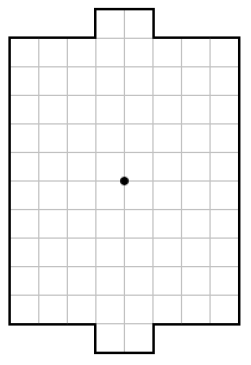
\includegraphics[width=0.2\textwidth]{board}
  \caption{Pusta plansza}
\end{figure}

Najczęściej stosowanym wymiarem planszy jest 8 na 10 kratek.
Przy krótszych bokach narysowane są dwie bramki o szerokości 2 kratek, w których gracze muszą umieścić piłkę.
Rozgrywka toczy się jedynie na przecięciach linii.
Środek planszy jest punktem startowym gry, do którego gracze dorysowują kolejne linie, oznaczające przemieszczenie piłki na sąsiednie pole. Każdy kolejny ruch zaczyna się w miejscu, w którym skończył się poprzedni, wzdłuż kratki lub po przekątnej. 

Ruchy nie mogą odbywać się po brzegu planszy ani wzdłuż odcinków, po których wcześniej piłka była już prowadzona.
Możliwe jest odbijanie się, które polega na wykonaniu przez gracza dodatkowego ruchu. Następuje ono gdy ruch zostanie zakończony w miejscu, w którym kończy się już linia narysowana przez jednego z graczy lub na brzegu boiska. 

\begin{figure}[ht]
  \centering
  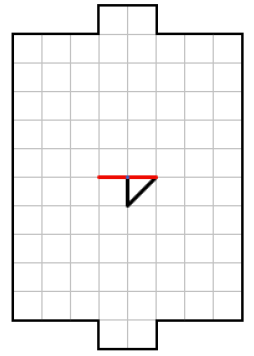
\includegraphics[width=0.2\textwidth]{odbicie}
  \caption{Odbicie (kolor czerwony)}
  \label{fig:odbicie}
\end{figure}

Gra kończy się w momencie gdy piłka znajdzie się w jednej z bramek.
Wówczas gracz, do którego należy dana bramka przegrywa. 
Gracz może również przegrać w wypadku gdy nie jest w stanie wykonać żadnego ruchu.

Do zapisu gry wykorzystuje się notację, w której każdy z ruchów określony jest liczbą naturalną od 0 do 7, gdzie 0 oznacza ruch w górę, a kolejne idą zgodnie z ruchem wskazówek zegara o 45 stopni. Ruchy oddziela się przerwą jedynie pomiędzy graczami. Przykładowo grze na rysunku \ref{fig:odbicie} odpowiada zapis: $ 1. \; 4 \;1 \; 2. \; 66 $, gdyż w rundzie turze zostały wykonane ruchy w dół (4), następnie do góry w prawo (1), a w drugiej -- podwójny ruch w lewo (6 i 6).

\begin{figure}[ht]
  \centering
  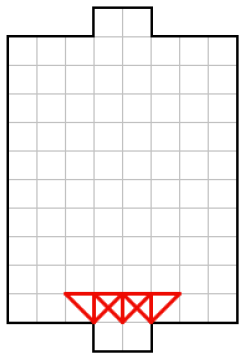
\includegraphics[width=0.2\textwidth]{zablokowanie}
  \caption{Zablokowana bramka}
\end{figure}
 
\section{Cel badawczy} 

% todo napisz wczesniej cos o AlphaGo

Celem mojej pracy jest zastosowanie algorytmu AlphaGo \cite{alphago2016, alphagozero}, który w 2016 zwyciężył podczas gry z mistrzem świata w Go, stając się najlepszym graczem i jednocześnie najbardziej zaawansowanym algorytmem uczenia ze wzmocnieniem, do wyuczenia agenta zdolnego do gry w piłkarzyki na kartce. Postaram się w niej dowiedzieć w jaki sposób hiperparametry wykorzystane w AlphaGo powinny zostać zaadaptowane do mojego problemu. 

Ponadto maszyny wykorzystywane do uczenia AlphaGo są rzędy wielkości lepsze od komputerów wykorzystywanych przez przeciętną osobę. Moje eksperymenty będą skupiały się również na tym które hiperparametry mogą zostać zredukowane, aby jednocześnie uzyskać wyniki w sensownym czasie oraz aby były one dla nas satysfakcjonujące.


\section{Wkład własny}

Za mój wkład uważam:

\begin{itemize}

\item Zastosowanie metod uczenia ze wzmocnieniem do piłkarzyków na papierze, które nie przyciągnęły do tej pory niczyjej uwagi,

\item Wyznaczenie które hiperparametry mogą zostać zredukowane, aby móc przeprowadzić eksperyment na przeciętnej maszynie,

\item Reimplementacja algorytmu wykorzystanego w AlphaGo oraz wyuczenie wag.

\end{itemize}

\section{Zarys pracy}

Pozostała część tekstu została podzielona na następujące rozdziały:
\begin{itemize}

\item W rozdziale drugim postaram wprowadzić czytelnika w zagadnienie uczenia ze wzmocnieniem, wyprowadzając podstawowe definicje oraz pojęcia, które wykorzystywane będą w dalszych częściach.

\item W rozdziale trzecim zaznajomię czytelnika z tematem głębokich sieci neuronowych, które stanowią dziś ogromną część uczenia maszynowego i cieszą się popularnością ze względu na swoje znakomite osiągnięcia.

\item W rozdziale czwartym wytłumaczę w jaki sposób połączyć ze sobą światy uczenia ze wzmocnieniem oraz głębokich sieci neuronowych, otrzymując w ten sposób głębokie uczenie ze wzmocnieniem, które odpowiedzialne jest obecnie za czołowe osiągnięcia w dziedzinie uczenia ze wzmocnieniem, takie jak autonomiczne samochody czy AlphaGo.

\item W rozdziale piątym opowiem o wykonanym przeze mnie eksperymencie uczenia się gry w piłkarzyki na kartce. Wyjaśnię w jaki sposób algorytm zdobywa doświadczenie potrzebne mu podczas uczenia się oraz w jaki sposób wygląda proces podejmowania decyzji oraz uczenia się.

\item Ostatni rozdział podsumowuje wykonaną pracę i zawiera wyciągnięte podczas niej wnioski.
\end{itemize}
 
\chapter{Uczenie ze Wzmocnieniem}\label{r:rl}

\section{Wprowadzenie}

Uczenie ze wzmocnieniem (ang. Reinforcement Learning, RL) \cite{Sutton, Szepesvari} jest działem uczenia maszynowego, zajmującym się sekwencyjnym podejmowaniem decyzji. Na proces uczenia składa się \emph{agent}, który uczy się podejmować decyzje oraz \emph{środowisko}, które stanowi cały świat zewnętrzy dla agenta. Interakcja między nimi polega na naprzemiennym wykonywaniu akcji przez agenta oraz prezentowaniu mu przez środowisko nowej sytuacji w której się znalazł i nagrody jaką otrzymał. Celem agenta jest maksymalizacja nagród, które otrzymuje.

Podczas procesu uczenia się, nigdy nie wskazujemy agentowi optymalnej akcji, a zamiast tego musi on sam do niej dojść. Stanowi to główną różnice pomiędzy uczeniem ze wzmocnieniem a uczeniem nadzorowanym (ang. Supervised Learning). Rozdział oparty jest na książce Suttona oraz Barto \cite{Sutton}.

\section{Dyskretny Proces Markowa}

Dyskretny Proces Markowa składa się z:
\begin{itemize}
\item zbioru stanów w których może znaleźć się agent, $ s \in \mathcal{S} $,
\item rozkładu stanu początkowego $\mathcal{D}$ nad zbiorem $\mathcal{S}$,
\item zbioru akcji możliwych do podjęcia przez agenta, $ a \in \mathcal{A} $
\item nagrody otrzymywanej przez agenta za każdym razem, gdy ten wykona jakąś akcje, $ R_t \in \mathbb{R} $
\item prawdopodobieństwa przejścia między stanami
$$ p(s'|s, a) = \mathbb{P}(S_{t+1} = s' \mid S_t = s, A_t = a)$$
\item współczynnik dyskontującego wartości nagród otrzymywanych w przyszłości $ \gamma \in [0, 1] $
\end{itemize}


\section{Wynik oraz epizody}

Interakcja między agentem a środowiskiem zachodzi w każdym, dyskretnym punkcie czasu $ t = 0, 1, 2, ... $. Znajdując się w punkcie czasu $t$, agent obserwuje stan $ S_t \in \mathcal{S} $, w którym się znajduję, na jego podstawie wykonuje akcję $ A_t \in \mathcal{A}(S) $, gdzie $ \mathcal{A}(s) $ jest zbiorem wszystkich akcji, które można wykonać znajdując się w stanie $S$. W kolejnym kroku dowiaduje się on jaką nagrodę $ R_{t+1} \in \mathbb{R} $ otrzymał i do jakiego stanu $ S_{t+1} $ się przeniósł. Stan w którym nasz agent rozpoczyna interakcje ze środowiskiem nazywamy \emph{początkowym} i jest on wyznaczany losowo przez środowisko na podstawie rozkładu $\mathcal{D}$, natomiast stany do których nasz agent się przenosi są zgodne z rozkładem prawdopodobieństwa przejścia między stanami. W wyniku otrzymujemy następujący ciąg stanów, akcji oraz nagród, zwany \emph{trajektorią}:

$$ S_0, A_0, R_1, S_1, A_1, R_2, ... $$


\begin{figure}[ht]
  \centering
  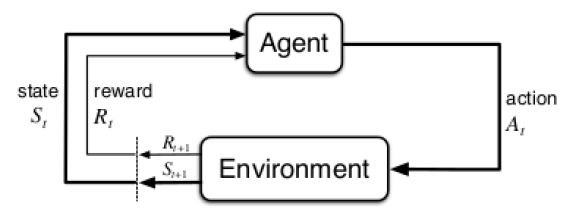
\includegraphics[width=0.5\textwidth]{agent_env_interaction}
  \caption{Interakcja między agentem a środowiskiem jako Dyskretny Proces Markowa. \cite{Sutton}}
\end{figure}

Najprostszym typem środowisk są te w których ilość kroków jest z góry ograniczona. Pojedynczy ciąg interakcji nazywamy wówczas \emph{epizodem}, a ostatni stan obserwowany przez agenta -- \emph{stanem terminalnym}. W tym wypadku epizody są od siebie niezależne, mogą się one kończyć w różnych stanach oraz po różnej ilości kroków. 

Celem naszego agenta jest maksymalizacja wartości oczekiwanej sumy nagród, które zdobędzie on w przyszłości. Określmy ją jako \emph{wynik}, $ G_t $, który zdefiniowany jest następująco:

$$ G_t = R_{t+1} + R_{t+2} + R_{t+3} + ... + R_{T-1} = R_{t+1} + G_{t+1} $$

gdzie $T$ jest końcem epizodu, a $t$ indeksem czasu. Sam problem nauczenia naszego agenta w jaki sposób powinien on podejmować decyzje, aby osiągnąć najwyższy wynik, nazywamy \emph{epizodycznym zadaniem}.

Możemy również spotkać się ze środowiskami, z którymi interakcja przebiega nieprzerwanie. Mamy wówczas do czynienia z \emph{ciągłym zadaniem}. Wprowadzamy wówczas koncepcje \emph{dyskontowania} wyniku, który definiujemy następująco:

$$ G_t = R_{t+1} + \gamma R_{t+2} + \gamma^2 R_{t+3} + ... = 
\sum_{k=0}^{\infty} \gamma^k R_{t+k+1} $$

gdzie $ \gamma \in [0, 1) $. Wymagany go aby zapewnić ograniczoność wyniku.


\section{Strategia}

Strategia jest funkcją która każdemu stanowi przyporządkowuje akcję. Może być ona deterministyczna, $ \pi(s) $, lub też stochastyczna, $ \pi(a \mid s) $, i wówczas stanowić rozkład prawdopodobieństwa wszystkich akcji dla ustalonego stanu. Metody uczenia ze wzmocnieniem określają w jaki sposób strategia jest modyfikowana na podstawie doświadczenia zbieranego przez agenta.

\section{Funkcja Wartości}

Posiadając strategię, możemy chcieć się dowiedzieć jaką nagrodę uzyska agent, który będzie się nią kierował. W tym celu definiujemy \emph{funkcję wartości stanu} (ang. Value Function), którą oznaczamy jako $ v_{\pi}(s) $ dla ustalonej strategii $ \pi $. Definiujemy ją jako:

$$ v_{\pi}(s) = \mathbb{E}_{\pi}[G_t \mid S_t = s] = \mathbb{E}_{\pi} \Bigg[ \sum_{k=0}^{\infty} \gamma^k R_{t+k+1} \bigg| S_t = s \Bigg] $$

gdzie $ \mathbb{E}_{\pi} $ jest wartością oczekiwaną wyniku $ G_t $ agenta, który w momencie $t$ wykona akcje $s$, a następnie postępuje zgodnie ze strategią $\pi$.

Podobnie definiujemy wartość wybrania akcji $a$, gdy znajdujemy się w stanie $s$ oraz podążamy zgodnie ze strategią $\pi$, oznaczaną jako $q_{\pi}(s, a)$. Jest ona wartością oczekiwaną z sytuacji w której rozpoczynamy w stanie $s$, wykonujemy akcję $a$, po czym wszystkie kolejne akcje wykonujemy zgodnie ze strategią $\pi$. Funkcję tę nazywamy \emph{funkcją wartości akcji} lub \emph{Q-funkcją}.

$$ q_{\pi}(s, a) = \mathbb{E}_{\pi}[G_t \mid S_t = s, A_t = a] = \mathbb{E}_{\pi} \Bigg[ \sum_{k=0}^{\infty} \gamma^k R_{t+k+1} \bigg| S_t = s, A_t = a \Bigg] $$

\section{Optymalność strategii oraz funkcji wartości}

Podczas rozwiązywania problemu uczenia ze wzmocnieniem staramy się znaleźć strategię, której przestrzeganie przyniesie naszemu agentowi możliwie największą nagrodę. Będziemy mówić że strategia $\pi$ jest lepsza lub równa strategii $\pi'$, wtedy i tylko wtedy gdy oczekiwana nagroda dla niej jest większa lub równa niż dla $\pi'$ w każdym stanie należącym do przestrzeni stanów. Zawsze istnieje strategia, która jest lepsza lub równa od wszystkich innych i nazywamy ją \emph{optymalną strategią}. Może istnieć wiele różnych od siebie optymalnych strategii, dla uproszczenia wszystkie oznaczamy tak samo jako $\pi_{\ast}$. Każda z nich posiada identyczną funkcję wartości stanu, nazywamy ją \emph{optymalną funkcją wartości stanu}. Spełnia ona własność:

$$ v_{\ast}(s) = \max_{\pi} v_{\pi}(s) $$

dla każdego stanu $s \in \mathcal{S}$. Podobnie współdzielą one \emph{optymalną funkcję wartości akcji}, $q_{\ast}$, która spełnia:

$$ q_{\ast}(s, a) = \max_{\pi} q_{\pi}(s, a) $$

dla każdego stanu $s \in \mathcal{S}$ oraz akcji $a \in \mathcal{A}$.

Ponadto optymalną funkcję wartości stanu możemy zdefiniować odwołując się do funkcji wartości akcji w następujący sposób:

$$ v_{\ast}(s) = \max_{a \in \mathcal{A}} q_{\pi_{\ast}}(s) $$

Podstawową własnością spełnianą przez funkcję wartości jest \emph{równanie Bellmana}. Dla dowolnej strategii $\pi$ oraz stanu $s$ zachodzi:

\begin{align}
v_{\pi}(s) &= \mathbb{E}_{\pi}[G_t \mid S_t = s]  \nonumber \\
&= \mathbb{E}_{\pi}[R_{t+1} + \gamma R_{t+2} + \gamma^2 R_{t+3} + ... \mid S_t = s]  \nonumber \\
&= \mathbb{E}_{\pi}[R_{t+1} + \gamma (R_{t+2} + \gamma R_{t+3} + ... ) \mid S_t = s]  \nonumber \\
&= \mathbb{E}_{\pi}[R_{t+1} + \gamma G_{t+1} \mid S_t = s] \nonumber \\
&= \sum_a \pi(a \mid s) \sum_{s'} \sum_r p(s', r \mid s, a) \Big(r + \gamma \mathbb{E}_{\pi}[G_{t+1} \mid S_{t+1} = s' ]\Big) \nonumber \\
&= \sum_a \pi(a \mid s) \sum_{s', r} p(s'\mid s, a) \Big(r + \gamma v_{\pi}(s') \Big)
\end{align}

gdzie $ p(s', r \mid s, a) $ jest prawdopodobieństwem przejścia do stanu $s'$ i  otrzymania nagrody $r$ po wykonaniu akcji $a$ w stanie $s$.

Na podstawie własności optymalnych funkcji wartości oraz równania Bellmana możemy wyprowadzić \emph{równania optymalności Bellmana} \cite{bellman1954, bellman1957}, bez odwoływania się przy tym do żadnej strategii. Pierwsze z nich odnosi się do funkcji wartości stanu:

\begin{align}
v_{\ast}(s) &= \max_{a \in \mathcal{A}} q_{\pi_{\ast}}(s, a) \nonumber \\
&= \max_a \mathbb{E}_{\pi}[G_t \mid S_t = s, A_t = a]  \nonumber \\
&= \max_a \mathbb{E}_{\pi}[R_{t+1} + \gamma G_{t+1} \mid S_t = s, A_t = a] \nonumber \\
&= \max_a \mathbb{E}[R_{t+1} + \gamma v_{\pi_{\ast}}(S_{t+1}) \mid S_t = s, A_t = a] \nonumber \\
&= \max_a \sum_{s', r} p(s', r \mid s, a) \Big[r + \gamma v_{\ast}(s') \Big]
\end{align}

Natomiast drugie zdefiniowane jest dla funkcji wartości akcji:

\begin{align}
q_{\ast}(s, a) &= \mathbb{E}[R_{t+1} + \gamma \max_{a'} q_{\ast} (S_{t+1}, a') \mid S_t = s, A_t = a] \nonumber \\
&= \sum_{s', r} p(s', r \mid s, a) \Big[r + \gamma \max_{a'} q_{\ast} (s', a') \Big]
\end{align}

\section{Metody uczenia ze wzmocnieniem}

Metody rozwiązywania problemu uczenia ze wzmocnieniem możemy podzielić ze względu na to czy wykorzystują one model środowiska. Metody \emph{model-based} wymagają od nas \emph{modelu} środowiska wykorzystywanego przez agenta aby przewidzieć w jaki sposób otoczenie będzie zachowywało się w odpowiedzi na wykonywane przez niego akcje.
Dzięki temu możliwe jest \emph{planowanie}, które pozwala na przewidywanie stanów oraz nagród na wiele kroków wprzód. Tego typu problemy możemy spotkać przy okazji nauki naszego agenta gry w Go\cite{alphago2016, alphagozero}, gdzie środowisko imitowane jest przez niego samego, podczas gdy gra on sam ze sobą. W ten sposób przewiduje on jakie akcje podejmie przeciwnik w odpowiedzi na jego ruchy, dzięki czemu może on podejmować jeszcze lepsze decyzje.
Drugą klasą algorytmów są metody \emph{model-free}, w których agent posiada jedynie strategię oraz funkcję wartości, a samo zachowanie środowiska jest dla niego nieznane i może on obserwować jedynie bezpośrednie skutki swoich działań. Z takimi problemami spotykamy się np. w przypadku gry naszego agenta na Atari, gdzie nie próbujemy dowiedzieć się jakie prawa rządzą poszczególnymi grami, a zamiast tego po prostu dajemy naszemu agentowi grać.

\subsection{Metody Monte Carlo}

Metody Monte Carlo korzystają z idei \emph{iteracji strategii} \cite{policy-iteration}, która składa się z dwóch, przeplatających się ze sobą procesów. Pierwszy krok, nazywany \emph{krokiem ewaluacji strategii}, polega na aproksymacji funkcji wartości na podstawie strategii, wykorzystywanej przez agenta. Z kolei w drugim kroku ulepszamy obecną strategię, przy użyciu wcześniej uzyskanej funkcji wartości. Nazywamy go \emph{krokiem ulepszania strategii}.

W przypadku metod Monte Carlo, ewaluacje strategii wykonujemy poprzez próbkowanie kolejnych trajektorii, a następnie wyliczanie średniego wyniku dla każdego ze stanów, bądź każdej pary stan-akcja. Zbierana przez nas historia akcji w postaci trajektorii nazywamy \emph{doświadczeniem} agenta. Najprostszy sposób aktualizacji funkcji wartości może wyglądać następująco:

$$ v(s_t) \leftarrow v(s_t) + \alpha \big[G_t - v(s_t)\big] $$

gdzie $G_t$ oznacza wynik agenta następujący po czasie $t$, a $\alpha$ parametrem wpływającym na szybkość uczenia się.

Ulepszanie strategii następuje poprzez zachłanny wybór najlepszej akcji dla każdego ze stanów, na podstawie wyuczonej funkcji wartości akcji. Jednak w przypadku takiego doboru strategii, skazujemy się na deterministyczną strategię, która nie jest w stanie odkrywać nowych, potencjalnie lepszych akcji, gdyż cały czas wybierać będzie ona te same akcje. 

Aby utrzymać eksploracje nowych akcji oraz stanów, wprowadzamy pojęcie \emph{$\varepsilon$--zachłannej} strategii, która z wysokim prawdopodobieństwem wykonuje akcję, która maksymalizuje wartość funkcji wartości akcji, a od czasu do czasu wykonuje losową akcję. Dzięki temu utrzymujemy stały poziom eksploracji, a przy niewielkich założeniach dla epsilona strategia zbiega do optymalnej.

$$
\pi(a \mid s) =
\begin{cases}
    1 - \epsilon + \epsilon/\lvert \mathcal{A}(s) \rvert & \text{if } a = a^\ast \\
    \epsilon/\lvert \mathcal{A}(s) \rvert,              & \text{if } a\neq a^\ast
\end{cases}
$$

Metody Monte Carlo cierpią z powodu wysokiej wariancji podczas uczenia, przez co potrzeba bardzo wielu iteracji, aby agent mógł wyuczyć się sensownej strategii, co z kolei wiąże się z ogromnym kosztem ponoszonym na uczenie. Metody Monte Carlo są przykładem metod model-free.

\subsection{Temporal-Difference Learning} 

Bardzo istotnym podejściem wykorzystywanym w uczeniu ze wzmocnieniem jest \emph{temporal-difference} learning (TD Learning) \cite{TD}. Podobnie do metod Monte Carlo wykorzystuje ono doświadczenie agenta bez potrzeby wykorzystania modelu środowiska. Nie jest wymagane jednak oczekiwanie na zakończenie epizodu, aby zaktualizować wartość funkcji wartości, a zamiast tego aktualizacje mogą następować po wykonaniu pojedynczego kroku. Aktualizacja funkcji wartości w przypadku TD learning może wyglądać następująco:

$$ V(S_t) \leftarrow V(S_t) + \alpha \big[R_{t+1} + \gamma V(S_{t+1}) - V(S_t) \big] $$

Sposób tej aktualizacji nazywany jest \emph{TD(0)} lub też \emph{jedno--krokowym} TD, a sam wyraz o który aktualizowana jest wartość:

$$ \delta_t = R_{t+1} + \gamma V(S_{t+1}) - V(S_t) $$

nazywamy \emph{błędem TD}.

\begin{figure}[ht]
  \centering
  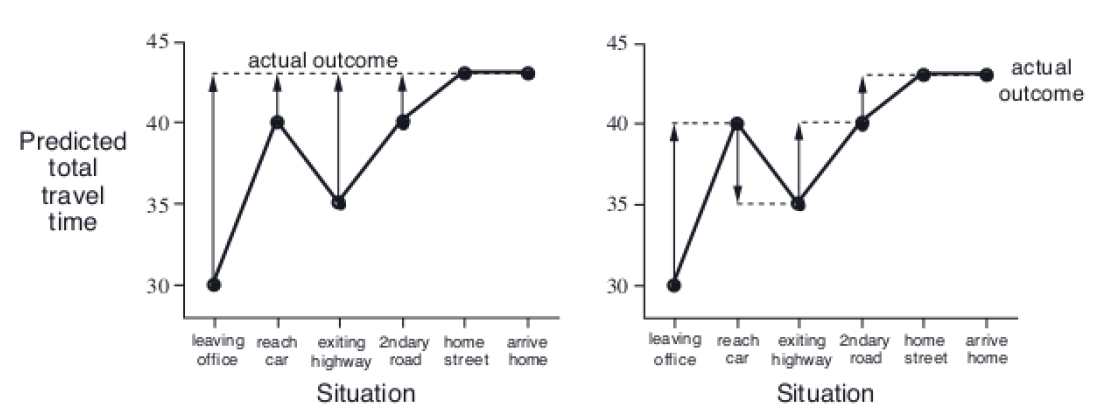
\includegraphics[width=1.0\textwidth]{mc_td}
  \caption{Porównanie aktualizacji funkcji wartości w przypadku metod Monte Carlo (po~lewej) oraz metod TD (po~prawej). \cite{Sutton}}
\end{figure}

Metody w uczeniu ze wzmocnieniem dzielimy również ze względu na to czy ewaluacja strategii przebiega przy użyciu strategii, która została wykorzystana podczas generowania trajektorii. Metody ewaluujące tę samą strategię nazywamy \emph{on-policy}, natomiast te które działają na różnych strategiach nazywamy \emph{off-policy}.

Dwoma podstawowymi algorytmami zaliczającymi się do TD learning jest \emph{SARSA (State-Action-Reward-State-Action} \cite{SARSA} oraz \emph{Q-Learning} \cite{Q-learning}.

SARSA jest przykładem metody on-policy, która wykorzystuje funkcję wartości akcji, zamiast funkcji wartości stanu. W przypadku tej metody aktualizacja funkcji wartości akcji jest następująca:

$$ Q(S_t, A_t) \leftarrow Q(S_t, A_t) + \alpha \big[R_{t+1} + \gamma Q(S_{t+1}, A_{t+1}) - Q(S_t, A_t) \big] $$

Aktualizacja ta zachodzi dla każdego nieterminalnego stanu $S_t$, a w przypadku gdy $S_{t+1}$ jest terminalny, to $ Q(S_{t+1}, A_{t+1}) $ definiujemy jako zero. Cały proces zależny jest od piątki $ (S_t, A_t, R_{t+1}, S_{t+1}, A_{t+1}) $, skąd pochodzi nazwa algorytmu \emph{SARSA}.

Q-Learning natomiast jest przykładem metody off-policy, w której aktualizacja Q-funkcji przebiega następująco:

$$ Q(S_t, A_t) \leftarrow Q(S_t, A_t) + \alpha \big[R_{t+1} + \gamma \max_a Q(S_{t+1}, a) - Q(S_t, A_t) \big] $$

W ten sposób uczona przez nas funkcja $Q$ bezpośrednio aproksymuje $Q_\ast$, niezależnie od tego jaka strategia jest przez nas wykorzystywana do wybierania kolejnych akcji.

\subsection{Algorytmy Rollout}

Metody \emph{model-based}, wykorzystujące wymodelowane środowisko, opierają się na planowaniu kolejnych ruchów, które w przyszłości podejmie nasz agent. Główną metodą planowania jest \emph{planowanie w momencie podjęcia decyzji}, które skupia się na podejmowaniu decyzji po znalezieniu się w konkretnym stanie $S_t$, a więc na wyborze akcji $A_t$. Najważniejszy dla nas wówczas jest stan, w którym się znaleźliśmy, mniej natomiast te odległe lub już odwiedzone. 

Algorytmy typu rollout są algorytmami planowania w momencie podjęcia decyzji  i bazują na bardzo podobnej zasadzie co metody Monte Carlo. Przybliżają one funkcję wartości akcji dla obecnego stanu, za pomocą symulowania kolejnych trajektorii, wykorzystując do tego strategię podstawową. Ich celem jednak nie jest znalezienie optymalnej strategii $\pi_\ast$ czy też funkcji $q_\ast$, a zamiast tego służą nam do stworzenia \emph{strategii rollout} za każdym razem gdy znajdziemy się w jakimś stanie. Otrzymane w ten sposób strategie są lepsze od wyjściowych, możemy więc traktować je jako metodę na ulepszanie posiadanej przez nas już strategii podstawowej.

\subsection{Monte Carlo Tree Search}

Przeszukiwanie drzew metodą Monte Carlo, czyli \emph{Monte Carlo Tree Search (MCTS)} \cite{MCTS} opiera się na algorytmach rollout i jest wykorzystywany między innymi w takich programach jak AlphaGo\cite{alphago2016, alphagozero}. 
Rozszerza on pomysł opisany w poprzedniej sekcji o przechowywanie i aktualizację funkcji wartości akcji dla kolejnych ruchów, zamiast jedynie dla stanu w którym znajduje się agent. W tym celu tworzone jest drzewo, ukorzenione w obecnym stanie, które wraz z kolejnymi symulacjami się rozszerza i dokładniej aproksymuje Q funkcję. Dla stanów obecnych w drzewie, decyzję podejmujemy na podstawie funkcji wartości zawartej w węzłach drzewa, a dla stanów poza drzewem wykorzystujemy podstawową strategię. Strategię wytworzoną w ten sposób nazywamy \emph{strategią drzewa}.

Pojedyncza iteracja MCTS dzieli się na cztery kroki:

\begin{enumerate}
\item \textbf{Wybór.} Wybierane są kolejne stany należące do drzewa na podstawie strategii utworzonej z wartości funkcji akcji, która zdefiniowana jest przez krawędzie grafu. Przejście przez drzewo rozpoczyna się w korzeniu, a kończy w liściu drzewa.
\item \textbf{Rozwinięcie.} Drzewo jest rozszerzane w liściu, który został osiągnięty w poprzednim kroku, poprzez dodanie nowych węzłów jako dzieci dla tego liścia. Nowe węzły reprezentują stany, które wcześniej nie były obecne w drzewie.
\item \textbf{Symulacja.} Zaczynając w węźle wybranym w pierwszym punkcie, rozpoczynana jest symulacja na podstawie strategii podstawowej. W wyniku otrzymujemy trajektorię, której pierwsze ruchy zostały wybrane za pomocą strategii drzewa, a pozostałe -- strategii podstawowej.
\item \textbf{Aktualizacja węzłów.} Wynik agenta jest propagowany wstecz do aktualizacji istniejących węzłów. Proces ten dotyczy jedynie stanów, które znajdują się w drzewie.
\end{enumerate}


\begin{figure}[ht!]
  \centering
  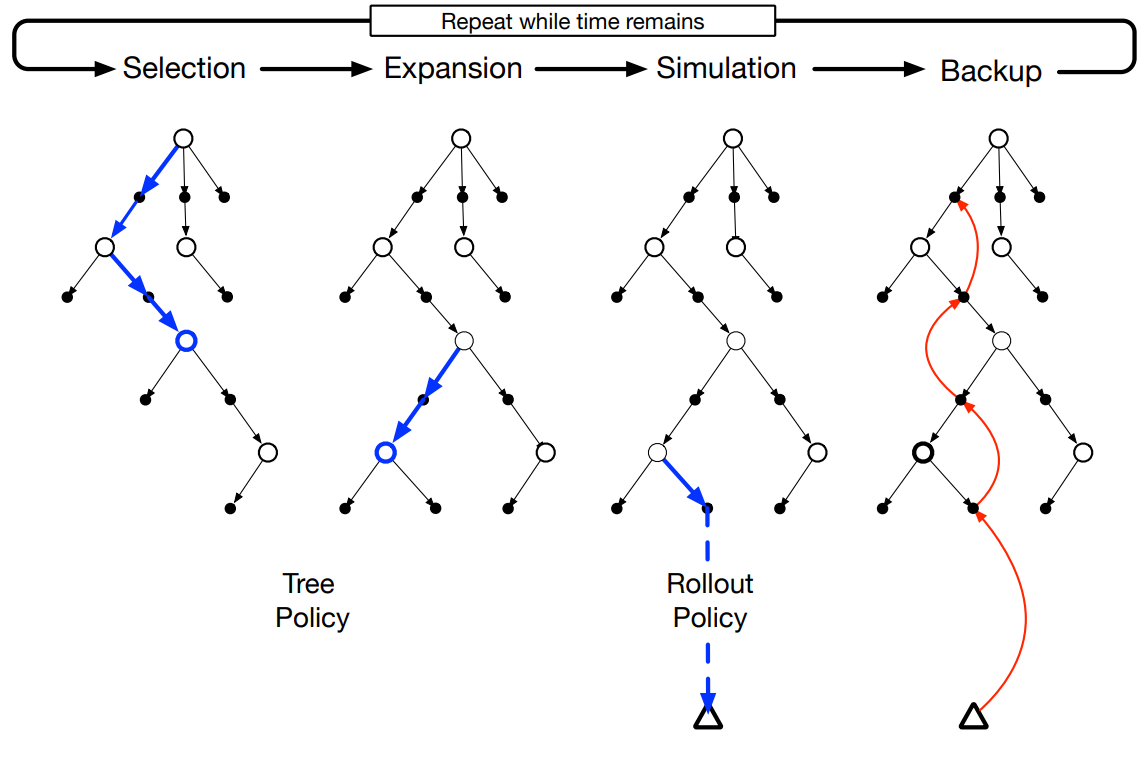
\includegraphics[width=0.85\textwidth]{mcts}
  \caption{Kolejne kroki podczas rozwijania drzewa w MCTS. \cite{Sutton}}
\end{figure}


\section{Podsumowanie}

W tym rozdziale zaprezentowane zostały podstawowe podejścia oraz koncepcje stosowane w uczeniu ze wzmocnieniem. Podczas tworzenia programów rozwiązujących gry strategiczne na planszy, jakimi są piłkarzyki na kartce czy Go, będziemy ze sobą łączyć te techniki, wzbogacając je dodatkowo o sieci neuronowe. W kolejnym rozdziale bliżej przyjrzymy się sieciom neuronowym, aby zrozumieć w jaki sposób one działają i jak możemy zastosować je do rozwiązania naszego problemu.

\chapter{Głębokie Sieci Neuronowe}

Ostatnio bardzo często mamy okazję słyszeć o Sztucznych Sieciach Neuronowych \cite{dlbook}. Ponownie stały się one popularne wśród społeczności sztucznej inteligencji i obecnie osiągają najlepsze wyniki w bardzo wielu dziedzinach. Stało się to między innymi za sprawą rozwoju komputerów, które są obecnie w stanie wykonywać ogromne ilości obliczeń. Sieci neuronowe pozwalają nam na tworzenie autonomicznych pojazdów \cite{sdc1, sdc2}, rozpoznawać obrazy lepiej od ludzi \cite{resnet, resnext} czy pokonać mistrza świata w Go\cite{alphago2016, alphagozero}. 

Głębokie Sieci Neuronowe mają zdolność do tworzenia aproksymacji nieliniowych funkcji na podstawie danych. Ponadto w porównaniu do innych modeli uczenia maszynowego, nie wymagają one ręcznego tworzenia cech na podstawie danych, a zamiast tego same tworzą własną reprezentacje. Dzięki temu ograniczają one wymaganą interakcje z modelem, przy jednoczesnej poprawie jakości uzyskiwanych cech.

\section{Sieci jednokierunkowe}

Głębokie sieci jednokierunkowe (ang. Deep Feedforward Networks), zwane również wielowarstwowym perceptronem (ang. Multilayer Perceptron), są podstawowym modelem głebokiego uczenia. Ich zadaniem jest przybliżanie funkcji $ y = f^{\ast}(x) $, która dla danych wejściowych $x$ przyporządkowuje decyzję bądź wartość $y$. Sieć jest wówczas funkcją $ y = f(x; \theta) $ parametryzowaną przez wektor $\theta$ i uczy się na podstawie danych.

Sieci neuronowe nazywane są sieciami, gdyż są one złożeniem wielu funkcji ze sobą, przez co informacje przepływają kolejno przez wszystkie z nich. Możemy je reprezentować jako acykliczny graf, który definiuje kolejne kroki wykonywanych obliczeń. Przykładowo możemy złożyć ze sobą dwie funkcje $ f(x) = f^{(2)}(f^{(1)}(x)) $, otrzymując sieć w której $f^{(1)} $ jest pierwszą warstwą, a $ f^{(2)} $ -- drugą. Ilość składanych ze sobą warstw nazywamy \emph{głębokością} sieci, ostatnią warstwę -- \emph{warstwą wyjściową}, a pozostałe warstwy -- \emph{ukrytymi warstwami}. 

W sieciach jednokierunkowych przepływ informacji występuje w jednym kierunku, a więc każda z warstw jest zależna jedynie od poprzednich. Nie występuje w nich sprzężenie zwrotne, które jest charakterystyczne dla rekurencyjnych sieci neuronowych.

Sztuczne sieci neuronowe swoją budową bazują na prawdziwych sieci neuronowych, które występują w mózgu. Warstwy sieci scharakteryzowane są przez \emph{szerokość}, która mówi o rozmiarze wektora produkowanego przez odpowiadającą jej funkcję. Każdy element wektora może pełnić wówczas funkcję analogiczną do neurona, który zbiera wszystkie informacje z poprzedniego wektora i tworzy na ich podstawie pewną wartość. Szerokość warstwy jest więc również ilością neuronów w niej zawartych. Wszystkie neurony w warstwie działają niezależnie od siebie. Pomimo jednak iż głębokie uczenie posiadają swoje korzenie w neuronaukach, to obecnie tworzone są one przez matematyków i inżynierów na podstawie ich własności matematycznych, a ich głównym celem nie jest naśladowanie działania mózgu.

\section{Budowa neuronu}

Każdy z neuronów na wejściu przyjmuje wektor $x$, który odpowiada poprzedzającej mu warstwie. Liczony jest jego iloczyn skalarny z wektorem wag $w$ i dodawane jest obciążenie $b$. Otrzymana wartość przekazywana jest do funkcji aktywacji $f$, a na końcu wyniki ze wszystkich neuronów są ze sobą konkatenowane w wektor, którego długość jest równa ilości neuronów w danej warstwie.

$$ y_i = f(\mathbf{x}^{T}\mathbf{w} + b) $$

Rolą funkcji aktywacji \cite{relu, activation-fn} w sieciach neuronowych jest wprowadzenie nieliniowości, dzięki którym możemy aproksymować dowolne funkcje. Najpopularniejszymi z nich są:

\begin{itemize}
\item Sigmoid:

$$ f(x) = \sigma(x) = \frac{1}{1 + e^{-x}}$$

\item Rectified Linear Unit (ReLU):

$$ f(x) = 
\begin{cases}
    x,              & \text{dla } x \geq 0\\
    0,              & \text{dla } x < 0
\end{cases}
$$

\item Tangens hiperboliczny:

$$ f(x) = \frac{e^x - e^{-x}}{e^x + e^{-x}} $$

\end{itemize}

W przypadku klasyfikacji, w której występuje wiele kategorii, wykorzystywana jest funkcja \emph{softmax}, która aplikowana jest od razu do całego wyjściowego wektora:


$$ f_i(x) = \frac{e^{x_i}}{\sum_k e^{x_k}} $$


\section{Uczenie sieci neuronowej}

Uczenie sieci neuronowej jest procesem optymalizacji, poleającym na minimalizacji bądź maksymalizacji pewnej funkcji $ f(x; \theta) $ za pomocą zmieniania wartośći $ \theta $. Funkcja $ f $ jest przez nas nazywana \emph{funkcją celu}, w przypadku minimalizacji często nazywana jest również \emph{funkcją kosztu}, \emph{funkcją straty} lub \emph{funkcją błędu}. 

Optymalizacja przebiega przy użyciu gradientu funkcji $ f $. Znając jego wartość możemy zmodyfikować $\theta$ o niewielki krok $ \alpha $, zwany \emph{krokiem uczenia} (ang. learning rate), aby odpowiednio zmniejszyć bądź zwiększyć wartość funkcji $ f $. 

$$ \theta_{i+1} = \theta_i - \alpha f'(x; \theta_i) $$

Metoda ta nazywana jest \emph{metodą gradientu prostego} (ang. Stochastic Gradient Descent, SGD) \cite{sgd}, a najczęściej stosowaną jej odmianą jest \emph{mini-batch SGD} \cite{mini-batch-sgd}, gdzie gradient liczony jest dla kilkudziesięciu przykładów z danych jednocześnie, po czym jest uśredniany. Przykłady pokazywane w jednym momencie sieci nazywane są \emph{partią} (ang. batch), a jedna iteracja w której sieć widzi wszystkie batche dokładnie raz, nazywana jest epoką.

Podczas tworzenia modelu możemy natrafić na pojęcia \emph{parametrów} oraz \emph{hiperparametrów}. Poprzez parametry sieci rozumiemy wektor cech $\theta$, który jest modyfikowany w procesie uczenia sieci, a inicjalizowany jest on losowo. Hiperparametrami natomiast nazywamy te czynniki, które ręcznie wyznaczamy przed rozpoczęciem procesu uczenia i są one przez nas arbitralnie wybierane. Nie jest możliwe ich uczenie się przez algorytm. Przykładami hiperparametrów modelu mogą być takie rzeczy jak głębokość sieci, szerokość sieci, krok uczący czy rozmiar batcha.

\begin{figure}[ht]
  \centering
  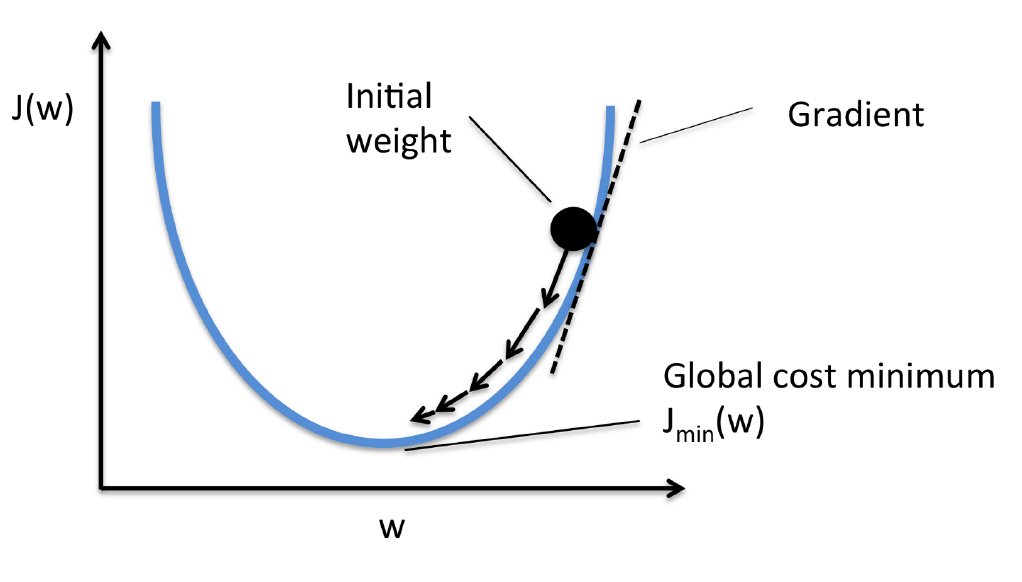
\includegraphics[width=0.5\textwidth]{sgd}
  \caption{Metoda stochastycznego gradientu prostego. \cite{sgd-img}}
\end{figure}

W zależności od rozwiązywanego przez nas zadania, dobiera się różne funkcje celu, a najpopularniejszymi z nich jest cross entropia (ang. Cross Entropy) w przypadku klasyfikacji:

$$ L_{log}(y, \hat{y}) = -\log\mathbb{P}(y | \hat{y}) = 
-\frac{1}{N} \sum_{i = 1}^N \sum_{k = 1}^M y_{i, k} \log \hat{y}_{i, k}
$$

gdzie $y$ to rzeczywista wartość funkcji, zwana również \emph{celem}, $\hat{y}$ to nasza predykcja, $N$ to rozmiar danych treningowych, a $M$ to liczba różnych klas. Dla modeli regresyjnych najczęściej wybieraną funkcją jest \emph{błąd średniokwadratowy} (ang. Mean Squared Error, MSE):

$$ L_{MSE}(y, \hat{y}) = \sum_{i = 1}^N (y_i - \hat{y}_i)^2$$

Różnica pomiędzy wykorzystaniem metod gradientowych optymalizacji w głębokim uczeniu maszynowym i klasycznym uczeniu maszynowym, jest brak wypukłości funkcji straty z powodu nieliniowości sieci neuronowych. Zbieżność danych metod do globalnego optimum nie jest gwarantowana, a jakość otrzymanego modelu jest zależna od parametrów początkowych. Powstało wiele metod aby unikać wpadnięcia w lokalne minima funkcji celu, powszechnie stosowanym sposobem jest modyfikacja sposobu aktualizacji wag, a przykładowymi i obecnie najpopularniejszymi algorytmami są \emph{Adam} \cite{adam} oraz \emph{RMSprop} \cite{rmsprop}. 

\section{Propagacja wsteczna}

W celu wykonania predykcji przy użyciu naszego modelu, musimy przekazać mu przykład, dla którego utworzy on estymację. Informacja o nim zostaje przekazywana przez kolejne warstwy, aby ostatecznie zwrócić jakiś wynik. Każdy kolejny krok wykonywanych obliczeń możemy utożsamić z przejściem po grafie, który definiuje w jaki sposób wygląda przepływ przez naszą sieć. Przetworzenie przykładu przez naszą sieć nazywamy wówczas \emph{propagacją} (ang. forward propagation). Otrzymana przez nas estymacja jest później wykorzystana w funkcji błędu. 

Algorytm propagacji wstecznej \cite{backprop} polega na przepływie sieci w przeciwnym kierunku, zaczynając od funkcji kosztu. Kolejne pochodne składające się na gradient liczone są przy pomocy metody łańcuchowej. Jest więc on algorytmem obliczającym gradient funkcji.

$$ \frac{dz}{dx} = \frac{dz}{dy} \frac{dy}{dx} $$
 

\section{Regularyzacja}

Częstym problemem występującym podczas uczenia sieci neuronowych oraz innych modeli uczenia maszynowego jest problem zbytniego dopasowania do danych (ang. overfitting). Występuje on gdy funkcja błędu na zbiorze treningowym osiąga znacząco niższy poziom niż na zbiorze testowym, który nie był obecny podczas uczenia się sieci. Zjawisko to oznacza brak dobrej generalizacji modelu poza zbiorem treningowym, co czyni go mało użytecznym dla nas. 
Podejmowane są różne kroki w celu zmniejszenia różnicy pomiędzy błędami obserwowanymi na obu tych zbiorach, a najpopularniejszym i najprostszym z nich jest regularyzacja parametrów. Zmniejsza ona teoretyczną pojemność modelu, co pozytywnie wpływa na jego jakość. Polega ona na dodaniu dodatkowego składnika do funkcji błędu, który odpowiada za zwiększanie jej wartości w zależności od parametrów sieci. Regularyzacja parametrów wykorzystywana jest również w prostszych modelach statystycznych, takich jak regresja liniowa \cite{lasso, ridge}. Zmodyfikowana funkcja straty jest wówczas postaci:

$$ L'(y, \hat{y}) = L'(y, f(x; \theta)) = L(y, f(x; \theta)) + \alpha \Omega(\theta) $$

gdzie $ \Omega(\theta) $ jest pewną normą wektora $ \theta $. Najpopularniejszą wyborem jest norma $ L^2 $.

Innymi znanymi metodami regularyzacji są takie rzeczy jak augmentacja danych czy dropout.

\section{Normalizacja batchów}

Uczenie głębokich sieci neuronowych okazuje się bardzo trudnym zadaniem. Aktualizacje warstw następują jednocześnie dla całej sieci, natomiast same gradienty liczone są przy założeniu że pozostałe warstwy pozostaną takie same. Zmiana parametrów może powodować modyfikację rozkładu wartości dowolnej z warstw, co z kolei może niekorzystnie wpływać na pozostałe. Wskutek tego musimy korzystać z małych learning rate, gdyż cały proces jest mocno niestabilny. Problem ten nazywany jest \emph{internal covariate shift} i rozwiązywany jest przez normalizację wyników z każdej warstwy. 

Normalizacja batchów (ang. batch normalization) \cite{batch-norm} polega na modyfikacji wyniku każdej z warstw, która wykonuje się przy każdej kolejnej propagacji partii. Po jej wykonaniu rozkład wartości z każdej z warstw ma zawsze tę samą średnią oraz wariancję.

$$ \mathbf{H'} = \frac{\mathbf{H} - \mathbf{\mu}}{\mathbf{\sigma}} $$

gdzie $ \mathbf{H} $ to wyjście z warstwy przed modyfikacją, a $ \mathbf{H'} $ -- po modyfikacji. Normalizacja batchów okazuje się również skuteczną metodą regularyzacji.

\section{Konwolucyjne Sieci Neuronowe}

\subsection{Wprowadzenie}

Konwolucyjne sieci neuronowe \cite{lecun-cnn, krizhevsky-cnn} są specjalnym typem architektury sieci, które wykorzystują przestrzenny charakter danych, które można reprezentować na kracie. Przykładem takich danych są zdjęcia, które są 2-wymiarowymi macierzami pikseli, oraz szeregi czasowe, które opisują pomiary oddalone od siebie jednakowymi odcinkami czasowymi. Obecnie konwolucyjne sieci neuronowe stanowią state-of-the-art w wielu dziedzinach uczenia maszynowego, a w szczególności we wszelkich zadaniach związanych z wizją komputerową. 

\subsection{Operacja Konwolucji}

Konwolucyjne sieci swoją nazwę zawdzięczają matematycznej operacji konwolucji, która w naszym wypadku jest wykonywana na dyskretnych wartościach:

$$ s(t) = (x * w)(t) = \sum_{a = -\infty}^{\infty} x(a)w(t - a) $$

Standardową terminologią dla sieci konwolucyjnych jest określanie funkcji $x$ jako \emph{wejścia}, funkcji $w$ jako \emph{filtr} lub \emph{jądro}, a wynik operacji jako \emph{wyjście}. Zarówno wejście, jak i wyjście, ze względu na swój przestrzenny charakter, nazywane są \emph{mapami cech}.

Często chcemy wykonywać operację konwolucji na wejściu o większej ilości wymiarów. W przpadku dwuwymiarowym wzór jest następujący:

$$ S(i, j) = (I * K)(i, j) = \sum_m \sum_n I(m, n) K(i - m, j - n) $$


\begin{figure}[ht!]
  \centering
  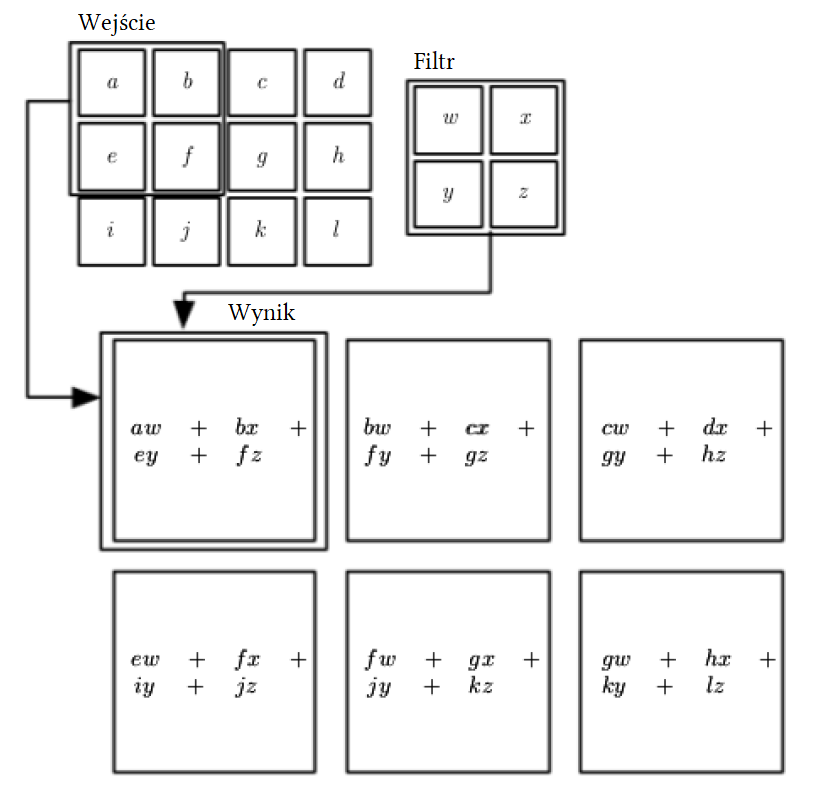
\includegraphics[width=0.6\textwidth]{konwolucja}
  \caption{Przykładowe wykonanie operacji konwolucji przy użyciu filtra 2 x 2. \cite{dlbook}}
\end{figure}

\subsection{Głębokie uczenie rezydualne}

Przez ostatnie lata architektury sieci neuronowych się pogłębiały, a uczenie ich stawało się co raz cięższe. Wykorzystanie \emph{rezydualnych bloków} \cite{resnet} okazało się częściowo rozwiązać ten problem i wspomóc proces uczenia się, a dzięki nim udało się trenować dużo głębsze sieci niż przed ich powstaniem. Ich wykorzystanie jest popularne w wielu obecnie stosowanych architekturach.

Przypuśćmy że oczekiwanym przez nas mapowaniem z warstwy konwolucyjnej byłaby funkcja $ \mathcal{H}(x) $. Rezydalne mapowanie polega na tym, aby bezpośrednie wyjście z warstwy dopasowywało się do funkcji $ \mathcal{F}(x) = \mathcal{H}(x) - x $, a oczekiwana wartość zostaje uzyskana poprzez późniejsze dodanie wejścia $x$. 

Zastosowanie tej transformacji okazuje się zdecydowanie poprawiać wyniki uczenia się sieci. Autorzy rezydualnego uczenia przypuszczają, że sieciom neuronowym dużo łatwiej jest nauczyć się rezydualnego mapowania, zamiast tego standardowego. W skrajnym przypadku gdyby optymalnym mapowaniem była identyczność, to wówczas dużo łatwiej jest wyuczyć się przekształcenia o zerowym wyjściu, niż identyczności.

\begin{figure}[ht!]
  \centering
  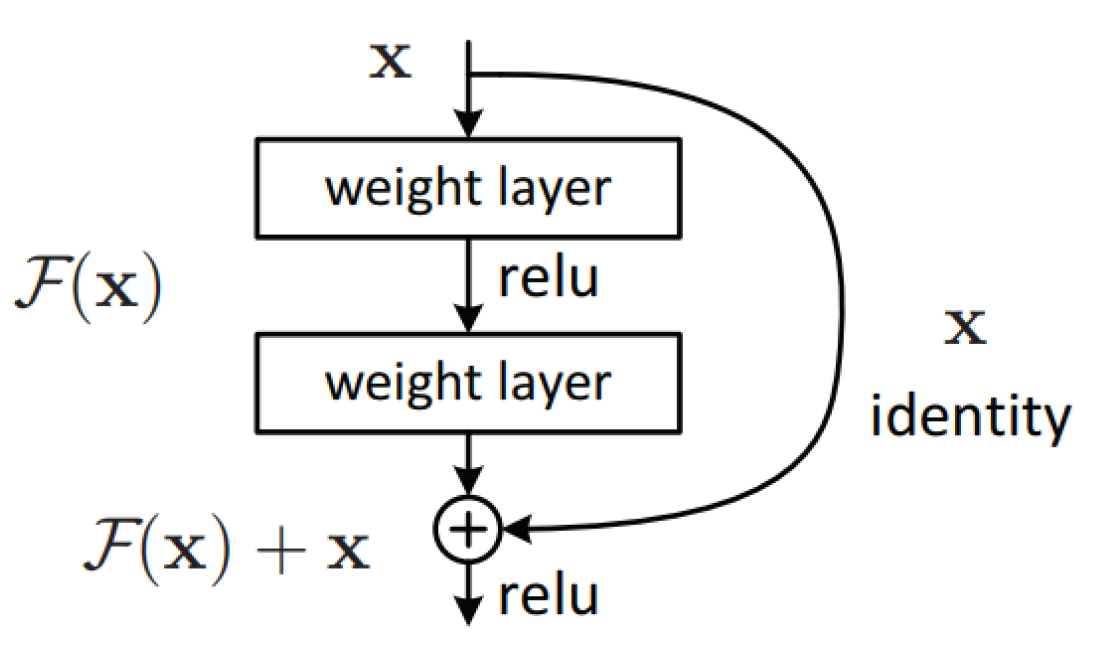
\includegraphics[width=0.6\textwidth]{res_block}
  \caption{Blok rezydualny. \cite{resnet}}
\end{figure}

Rezydualne uczenie zazwyczaj jest aplikowane do kilku ustawionych po sobie warstw. Razem z połączeniem od wejścia nazywamy je blokiem budującym i definiujemy go jako:

$$ y = \mathcal{F}(x; \theta) + x $$

Połączenie to nazywamy \emph{połączeniem skrótowym} (ang. shortcut connection). W przypadku gdy wymiar wejścia oraz wyjścia nie są sobie równe, to wykonujemy liniowe przekształcenie na wejściu, a blok definiujemy jako:

$$ y = \mathcal{F}(x; \theta) + W_sx $$

gdzie $W_s$ to macierz wag odpowiadających za projekcje na wymiar wyjściowy.

\section{Podsumowanie}

Głębokie sieci neuronowe obecnie są najlepszym typem modeli do aproksymacji dowolnych funkcji, gdyż możemy je tworzyć jedynie na podstawie surowych danych i nie jest wymagane ręczne tworzenie cech ani nie jest potrzebna specjalistyczna wiedza z zakresu problemu, który staramy się przy ich użyciu rozwiązać. Z tego powodu są one również bardzo popularne wśród metod uczenia ze wzmocnieniem, jako przybliżenia funkcji wartości oraz strategii, a ich zastosowanie w tej dziedzinie zostanie opisane w kolejnym rozdziale.

\chapter{Głębokie Uczenie ze Wzmocnieniem}

\section{Wprowadzenie}

Obecnie uczenie ze wzmocnieniem w głównej mierze opiera się na wykorzystaniu sieci neuronowych jako aproksymatory funkcji wartości lub strategii. Połączenie to pozwoliło nam na osiąganie niespotykanych dotąd wyników podczas rozwiązywania problemów takich jak gra w Dota 2 \cite{dota2} czy tworzenie autonomicznych samochodów \cite{sdc1, sdc2}. Dzięki zastosowaniu głębokiego uczenia jesteśmy w stanie radzić sobie z zadaniami, które charakteryzują się wielowymiarowością danych, a których rozwiązanie wcześniej było poza naszym zasięgiem.

Do głębokiego uczenia ze wzmocnieniem (ang. Deep Reinforcement Learning, DRL) zaliczamy takie metody jak \emph{głęboka Q-sieć} (ang. Deep Q-Network, DQN),  \emph{policy gradient} czy metody \emph{actor-critic}. Rozdział ten opisuje w jaki sposób uczenie ze wzmocnieniem łączone jest z głębokimi sieciami neuronowymi, prowadząc do najskuteczniejszych obecnie algorytmów. 

\section{Deep Q-Learning}

Jednym z ważniejszych algorytmów należących do tej kategorii jest \emph{głęboka Q-sieć} (DQN) \cite{dqn}, która jest połączeniem opisanego w pierwszym rozdziale \emph{Q-learningu} \cite{Q-learning} oraz sztucznych sieci neuronowych. Została ona wykorzystana w 49 różnych grach na Atari, osiągając w wielu z nich wyniki lepsze od ludzi. Sieć przyjmowała na wejściu jedynie obraz w postaci macierzy pikseli oraz wynik przez nią osiągany i na ich podstawie podejmowała decyzje. Nie tworzono ręcznie żadnych dodatkowych cech, a hiperparametry wykorzystane podczas uczenia były takie same dla każdej gry, co wskazuje na dobrą generyczność algorytmu.

W tym modelu sieć neuronowa pełni rolę funkcji wartości akcji, tj. Q-funkcji, a podczas uczenia minimalizowana była następująca funkcja straty:

$$ L_i(\theta_i) = \mathbb{E}_{s \sim \rho_{\pi(\cdot)}, a \sim \pi(\cdot)} \Big[ (y_i^2 - Q(s, a; \theta_i))^2 \Big] $$

gdzie $ y_i = \mathbb{E}_{s' \sim \mathcal{E}'} \big[ r + \gamma \max_{a'} Q(s', a'; \theta_{i - 1}) \mid s, a \big] $ jest celem funkcji w $i$-tej iteracji, $\pi(s \mid a)$ jest strategią utworzoną na podstawie Q-funkcji, $\rho_{\pi(\cdot)} $ jest rozkładem stanów podczas podążania zgodnie z strategią $\pi$. Aktualizacja wag sieci następuje zgodnie z gradientem powyższej funkcji, który jest postaci:

$$ \nabla_{\theta_i}L_i(\theta_i) = \mathbb{E}_{s, a \sim p(\cdot); s' \sim \mathcal{E}} 
\Big[ \Big( r + \gamma \max_{a'} Q(s', a'; \theta_{i - 1}) - Q(s, a; \theta_i) \Big) \nabla_{\theta_i} Q(s, a; \theta_i) \Big] $$

Funkcja straty jest optymalizowana przy pomocy metody gradientu prostego. W odróżnieniu od uczenia z nadzorem, zamiast niezależnych danych treningowych, dostajemy próbki zależne od wag $\theta$ i z tego powodu musimy korzystać z dodatkowych metod, dzięki którym pozbywamy się silnej korelacji pomiędzy próbkami. Korzystamy z metody zwanej \emph{powtórkami z doświadczenia} (ang. experience replay), która polega na zebraniu wielu trajektorii podczas procesu interakcji agenta ze środowiskiem i zapisywaniu ich jako powtórki w pamięci, a następnie próbkowane są losowo konkretne przykłady $(S_t, A_t, R_{t+1}, s_{t+1})$. Zastosowanie tej techniki sprawia iż zmniejszana jest wariancja podczas procesu uczenia się, dzięki czemu agent szybciej i stabilniej osiąga satysfakcjonujące nas rezultaty.


\section{Policy Gradient}

Metody \emph{policy gradient} \cite{policy-gradient-sutton} pozwalają nam na bezpośrednie modelowanie strategii agenta, bez konieczności korzystania z funkcji wartości. Możemy dzięki nim uzyskać strategię $\pi(a \mid s, \theta)$ parametryzowaną przez wektor $\theta$. Proces optymalizacji utworzonej w ten sposób strategii polega na maksymalizacji \emph{funkcji nagrody}, którą otrzymuje nasz agent, za pomocą \emph{wzrostowej metody gradientu prostego} (ang. gradient ascent). W przeciwieństwie do standardowej funkcji celu w głębokim uczeniu, którą zazwyczaj minimalizujemy, tym razem będziemy starać się maksymalizować tę funkcję, gdyż jest to nagroda otrzymywana przez naszego agenta.

Strategia może być dowolną funkcją $\pi(a \mid s, \theta)$, musi jednak być różniczkowalna względem parametru $\theta$, abyśmy mogli wykorzystać metody gradientowe podczas jej uczenia. Uzyskana w ten sposób strategia jest stochastyczna, co w wielu przypadkach jest przez nas wymaganym efektem. Najczęstszym wyborem funkcji $\pi$ są sieci neuronowe, które znane są z innych dziedzin uczenia maszynowego. Aktualizacja parametrów naszego modelu może przebiegać zgodnie ze wzorem:

$$ \theta_{i+1} = \theta_i + \alpha \nabla_{\theta}J , \quad
J = \mathbb{E}_{\pi} \Big( \sum_{k = 0}^{\infty} \gamma^k R_k \Big)
$$

\section{Algorytm REINFORCE}

Najprostszym przykładem metody policy gradient jest algorytm \emph{REINFORCE} \cite{reinforce}, który należy do metod Monte Carlo i opiera się na próbkowaniu kolejnych trajektorii przy użyciu strategii $\pi$, a następnie ulepszaniu jej na podstawie zebranego doświadczenia. \emph{Teoria Policy Gradient} daje nam przydatny wzór na proporcjonalność gradientu funkcji nagrody:

\begin{equation}\label{eq:pgt}
\nabla J(\theta) \propto \sum_s \mu(s) \sum_a q_{\pi} \nabla_{\theta} \pi(a \mid s, \theta)
\end{equation}

gdzie $\pi$ to strategia parametryzowana przez $\theta$, a $\mu$ jest \emph{rozkładem on-policy}, który mówi jaką część czasu spędzamy w każdym ze stanów. Formalnie definiujemy funkcję:

$$ \eta(s) = h(s) + \sum_{s'} \eta(s') \sum_{a} \pi(a \mid s') p(s \mid s', a) $$

gdzie $ h(s) $ oznacza prawdopodobieństwo rozpoczęcia się epizodu w stanie s, a zatem jest rozkładem początkowym stanów, a $p(s \mid s', a) $ jest prawdopodobieństwem przejścia ze stanu $s'$ do stanu $s$ po wykonaniu akcji $a$. Rozkład on-policy definiujemy wówczas jako:

$$ \mu (s) = \frac{\eta(s)}{\sum_s' \eta(s')} $$

Rozwijając dalej równanie \eqref{eq:pgt} otrzymujemy:

\begin{align*}
\nabla J(\theta) \propto & \sum_s \mu(s) \sum_a q_{\pi} \nabla_{\theta} \pi(a \mid s, \theta) \\
= & \mathbb{E}_\pi \Bigg[ \sum_{a} q_\pi (S_t, a) \nabla_\theta \pi(a \mid S_t, \theta) \Bigg]
\end{align*}

i w ten sposób pozbywamy się rozkładu $\mu$, który w przeciwnym wypadku musielibyśmy modelować lub znać. Zauważmy również że wystarcza nam proporcjonalność tego wyrażenia, gdyż aktualizacje parametrów będą wykonywane o pewien arbitralnie dobrany krok uczący $\alpha$, który niweluje uzyskaną nieproporcjonalność. Wykonując kolejne rachunki otrzymujemy: 

\begin{align*}
\nabla J(\theta) \propto  & \mathbb{E}_\pi \Bigg[ \sum_{a} \pi(a \mid S_t, \theta) q_\pi (S_t, a) \frac{\nabla_\theta \pi(a \mid S_t, \theta)}{\pi(a \mid S_t, \theta)} \Bigg] \\
= & \mathbb{E}_\pi \Bigg[ q_\pi(S_t, A_t) \frac{\nabla_\theta \pi(A_t \mid S_t, \theta)}{\pi(A_t \mid S_t, \theta)} \Bigg] \\ 
= & \mathbb{E}_\pi \Bigg[ G_t \frac{\nabla_\theta \pi(A_t \mid S_t, \theta)}{\pi(A_t \mid S_t, \theta)} \Bigg] 
\end{align*}

w pierwszym przejściu zamieniamy $a$ na obserwację $A_t \sim \pi$, a następnie korzystamy z własności $ \mathbb{E}_\pi \big[ G_t \mid S_t, A_t \big] = q_\pi(S_t, A_t) \big] $. W ten sposób otrzymujemy wyrażenie, które możemy wykorzystać do aktualizacji parametrów naszej sieci poprzez próbkowanie kolejnych trajektorii.

$$ \theta_{t+1} = \theta_t + \alpha G_t \frac{\nabla_\theta \pi(A_t \mid S_t, \theta)}{\pi(A_t \mid S_t, \theta)} $$

Często możemy również spotkać się z innym zapisem wyrażenia $  \frac{\nabla_\theta \pi(A_t \mid S_t, \theta)}{\pi(A_t \mid S_t, \theta)}$:

$$  \frac{\nabla_\theta \pi(A_t \mid S_t, \theta)}{\pi(A_t \mid S_t, \theta)} = \nabla_\theta \ln \pi(A_t \mid S_t, \theta) $$

Może się zdarzyć, np. w grach na Atarii, że dowolny ruch wykonany przez agenta przynosi sporą nagrodę, przez co podczas uczenia model będzie się starał zwiększać prawdopodobieństwa wszystkich tych ruchów. Aby wspomóc proces uczenia wprowadzamy pojęcie \emph{wartości bazowych}, $b(s)$, które odejmują od wszystkich nagród średnią oczekiwaną nagrodę ze stanu, w którym przebywa nasz aktor. W ten sposób będzie on zwiększał prawdopodobieństwa tylko tych akcji, które przynoszą lepszy wynik niż średni. Aktualizacja parametrów wygląda wówczas następująco:

$$ \nabla J(\theta) \propto \sum_s \mu(s) \sum_a \Big( q_\pi(s, a) - b(s) \Big) \nabla_\theta \pi(a \mid s, \theta) $$

których celem jest ograniczenie wariancji podczas uczenia się modelu. Warunkiem który funkcja $b$ musi spełniać jest jej niezależność od $a$, gdyż wtedy nie wprowadza ona dodatkowego obciążenia:

$$ \sum_a b(s) \nabla_\theta \pi(a \mid s, \theta) = b(s) \nabla_\theta \sum_a \pi(a \mid s, \theta) = b(s) \nabla_\theta 1 = 0 $$

Aktualizacja wag przyjmuje wówczas postać:

$$ \theta_{t+1} = \theta_t + \alpha \Big( G_t - b(S_t) \Big) \frac{\nabla_\theta \pi(A_t \mid S_t, \theta)}{\pi(A_t \mid S_t, \theta)} $$


Algorytm REINFORCE, podobnie jak wszystkie metody Monte Carlo, uczy się bardzo wolno, gdyż estymacje obarczone są wysoką wariancją. Rozwiązaniem tej niedogodności okazują się być modele przedstawione w kolejnej sekcji.

\section{Metody Aktor Krytyk}

Często nasz aktor może wykonać długą serię poprawnych ruchów, a dopiero na sam koniec popełnić błąd, który będzie kosztował go grę. W tym wypadku w metodzie REINFORCE prawdopodobieństwa wykonania wszystkich ruchów w trajektorii zostałyby obniżone. Metody aktor krytyk stanowią rozwiązanie dla tego problemu. Są one połączeniem modeli bazujących na strategii oraz tych bazujących na funkcji wartości. Strategia w tych metodach nazywana jest \emph{aktorem}, gdyż odpowiada ona za podejmowanie wykonywanych decyzji. Funkcja wartości nazywana jest \emph{krytykiem} i jej rolą jest ocenianie jakości akcji wykonywanych przez aktora. Parametry strategii są aktualizowane na podstawie estymacji wartości wykonywanych akcji za pomocą krytyka, zamiast wykorzystywać obarczone wysoką wariancją wyniki samych gier. W opisanym wyżej przykładzie obniżylibyśmy jedynie prawdopodobieństwo wykonania ostatniej akcji, która była dla nas niekorzystna, a pozostałe mogłyby pozostać bez zmian.

Jednym z prostszych algorytmów, który można przytoczyć jako przykład, jest jednokrokowa metoda aktor krytyk, która koncepcyjnie jest bardzo podobna do algorytmów takich jak TD(0) czy Sarsa. Pozwala ona na w pełni online algorytm uczenia, w którym zamiast korzystać z wyniku całego epizodu $G_t$, wykorzystujemy wynik jednokrokowy:

\begin{align*}
\theta_{t+1} =& \theta_t + \alpha \Big( G_t - \hat{v}(S_t, w) \Big) \frac{\nabla_\theta \pi(A_t \mid S_t, \theta)}{\pi(A_t \mid S_t, \theta)} \\
=& \theta_t + \alpha \Big( R_{t+1} + \gamma \hat{v}(S_{t+1}, w) - \hat{v}(S_t, w) \Big) \frac{\nabla_\theta \pi(A_t \mid S_t, \theta)}{\pi(A_t \mid S_t, \theta)} \\
=& \theta_t + \alpha \delta \frac{\nabla_\theta \pi(A_t \mid S_t, \theta)}{\pi(A_t \mid S_t, \theta)}
\end{align*}

gdzie $ \hat{v}(S_t, w) $ jest aproksymowaną funkcją wartości stanu, parametryzowaną przez wektor $w$, a $\delta$ jest TD-błędem. Funkcja wartości dla stanu $S_t$ jest początkowo odejmowana od wyniku $G_t$ jako wartość bazowa. 

\section{Podsumowanie}

Dla większości obecnie rozwiązywanych problemów przy użyciu uczenia ze wzmocnieniem, to modele głębokiego uczenia stanowią state-of-the-art i to na nich skupiona jest obecnie największa uwaga. W przypadku algorytmu AlphaGo Zero jego autorzy poszli o kolejny krok do przodu, włączając do modelu również przeszukiwanie drzewa rozgrywki, osiągając tym samym rezultaty które wcześniej wydawały się niemożliwe do uzyskania. Rozszerzenie tych metod zostanie opisane w kolejnym rozdziale, gdzie wykorzystując algorytm AlphaGo Zero staram się rozwiązać problem gry w piłkarzyki na papierze.

\chapter{Gra w piłkarzyki na kartce}

\section{Wprowadzenie}

Wielu specjalistów od dawna zajmuje się tworzeniem systemów grających w gry planszowe. Pierwszym krokiem milowym w rozwoju inteligentnych systemów było utworzenie Deep Blue \cite{deep-blue}, algorytmu potrafiącego grać w szachy, który w 1997 pokonał ówczesnego mistrza świata Garrego Kasparowa. Kolejnym celem stało się wówczas rozwiązania gry w Go, w której ilość ruchów na każdą rundę oraz długość rozgrywki są nieporównywalnie większe niż w przypadku szachów. W ostatnim czasie zespołowi z Deep Mind udało się utworzyć algorytm AlphaGo\cite{alphago2016}, który w roku 2016 pokonał mistrza świata Lee Sedol'a. Łączył on wszystkie znane do tamtej pory techniki wykorzystywane w uczeniu ze wzmocnieniem oraz głębokie uczenie. Natomiast w ubiegłym roku, 2017, został on rozwinięty do algorytmu AlphaGo Zero\cite{alphagozero}, który zupełnie generycznie, bez jakiejkolwiek wiedzy specjalistycznej, wykorzystując jedynie plansze jako wejście, osiągnął ponadludzkie zdolności gry w Go, wygrywając wszystkie gry przeciwko swojemu poprzedniku. 

Algorytm uczący agenta grającego w piłkarzyki na papierze jest w całości oparty na algorytmie AlphaGo Zero. Zmodyfikowana została jedynie architektura sieci oraz hiperparametry wykorzystane podczas uczenia.


\section{Reprezentacja danych}

Stan gry musi być w pewien sposób przez nas reprezentowany, aby sieć neuronowa mogła go przetworzyć i na jego podstawie podjąć decyzje. AlphaSoccer wykorzystuje sieć konwolucyjną, z tego powodu dane muszą być przedstawione jako mapa cech. 

W tym celu na planszy została wydzielona krata, w której komórce odpowiada pole, na którym znaleźć się piłka. Zatem jeśli nasze boisko zostało wyrysowane na kartce w kratkę o wymiarach $M \times N$, to nasza krata będzie wymiarów $(M + 1) \times (N + 1)$. Otrzymana przez nas krata odpowiada macierzy $\mathbb{R}^{n \times m}$ i stanowi ona pojedynczą warstwę w mapie cech. 

\begin{figure}[ht!]
  \centering
  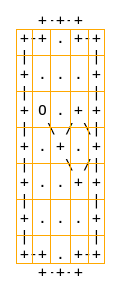
\includegraphics[width=35mm]{feature_map_grid}
  \caption{Plansza wraz z nałożoną kratą.}
\end{figure}

Na wejściową mapę cech składa się kilka warstw, które są ustawiane jedna na drugiej. Są to odpowiednio: 
\begin{itemize}
\item 8 warstw odpowiadających każdemu z kierunków,
$$ f(i, j, k) = 
\begin{cases}
    1,              & \text{gdy z miejsca (i, j) wychodzi linia w kierunku k}\\
    0,              & \text{wpp}
\end{cases}
$$
\item 1 warstwa odpowiadająca miejscom, od których można się odbić,
$$ f(i, j, w_o) = 
\begin{cases}
    1,              & \text{jeśli z (i, j) wychodzi linia w dowolną stronę} \\
    0,              & \text{wpp} 
\end{cases}
$$
\item 1 warstwa odpowiadająca pozycji piłki,
$$ f(i, j, w_p) = 
\begin{cases}
    1,              & \text{gdy piłka znajduje się na pozycji (i, j)}\\
    0,              & \text{wpp}
\end{cases}
$$

\item 1 warstwa odpowiadająca obciążeniu (bias),
$$ f(i, j, w_b) = 1 $$

Warto zauważyć, że wprowadzona została pewna redundancja, gdyż krawędzie są zawsze reprezentowane podwójnie, w obu stanach które dana krawędź łączy. Jest to celowe działanie i nic nie wskazuje na to, aby niekorzystnie wpływało na jakość modelu.

\begin{figure}
\centering
\setlength{\tabcolsep}{5mm}
\begin{tabular}{ccc}
  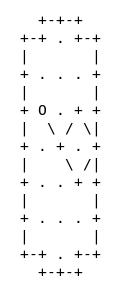
\includegraphics[width=35mm]{feature_map} & 
  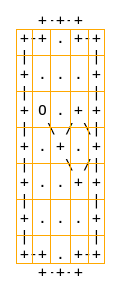
\includegraphics[width=35mm]{feature_map_grid} & 
  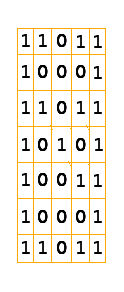
\includegraphics[width=35mm]{dots}\\
  Plansza z perspektywy & 
  Plansza wraz z & 
  Przykładowa warstwa w \\
  ludzkiego obserwatora. & nałożoną kratą. & 
  mapie cech -- warstwa odbić. \\
\end{tabular}
\caption{Reprezentacja danych.}
\end{figure}

\end{itemize}

\section{Algorytm przeszukujący drzewo gry}

Do podejmowania decyzji wykorzystywana jest sieć neuronowa $f_\theta$, która na wejściu wczytuje obecny stan planszy, a produkuje wektor prawdopodobieństw wykonania akcji oraz wartość stanu, która oznacza prawdopodobieństwo wygrania gry przez gracza z którego perspektywy wykonywany jest ruch, $f_\theta(s) = (p, v)$. W ten sposób funkcja wartości akcji oraz strategia łączona jest w jedną sieć neuronową, a konkretniej siecią konwolucyjną, złożoną z bloków rezydualnych, w której po ostatniej warstwie konwolucyjnej sieć rozbija się na dwie ścieżki, które kolejno są odpowiedzialne za strategię oraz funkcję wartości. W ten sposób te same cechy przestrzenne są wykorzystywane zarówno do wyboru akcji, jak i oceny wartości stanu. Zmniejsza to również złożoność obliczeniową.

Akcje podejmowane podczas rozgrywki są oparte na strategii drzewa, która budowana jest w trakcie rozgrywki. Agent przed wykonaniem każdego ruchu wykonuje szereg symulacji, polegających na rozgrywaniu gry z samym sobą. Wykorzystywany jest do tego algorytm MCTS, który wykorzystuje wyniki sieci neuronowej, aby uzyskać rozkład prawdopodobieństw akcji $\pi$, który jest lepszy od pierwotnego rozkładu $p$. 

Krawędzie w drzewie przeszukiwań odpowiadają parze $(s, a)$ -- stanu oraz akcji i przechowują one pierwotne prawdopodobieństwo wyboru tej akcji uzyskane z sieci neuronowej $P(s, a)$, licznik odwiedzin danej krawędzi $N(s,a)$, funkcję wartości akcji $Q(s,a)$ oraz sumę do tej pory zaobserwowanych funkcji wartości $W(s,a)$. 

\subsection{Przechodzenie ścieżki w drzewie}

Wybór akcji rozpoczyna się w korzeniu drzewa gry, reprezentującym stan w którym znajduje się agent. Wykonywane są kolejne symulacje, które polegają na wykonywaniu kolejnych akcji i przechodzeniu po drzewie, aż agent natrafi na liść. Wówczas wykonywane jest rozwinięcie danego liścia do nowego węzła i jego ewaluacja. Symulacje wykorzystują statystyki $\big(N(s,a), W(s,a), Q(s,a), P(s,a) \big)$. Akcjami wykonywanymi w kolejnych krokach są $a_t = \operatorname*{argmax}_a \big( Q(s_t, a) + U(s_t, a) \big)$. Funkcja $U$ zdefiniowana jest następująco:

$$ U(s,a) = c_{puct} P(s,a) \frac{\sqrt[]{\sum_b N(s,b)}}{1 + N(s,a)} $$ 

gdzie $c_{puct}$ jest to stała wyznaczająca poziom eksploracji podczas symulacji. W ten sposób początkowo zapewniona jest eksploracja, gdyż najpierw wybierane są akcje z wysokim początkowym prawdopodobieństwem, ostatecznie jednak preferowane są akcje z wysoką wartością funkcji wartości akcji.

\subsection{Rozwinięcie nowego węzła}

W momencie gdy algorytm przechodzenia drzewa natrafi na liść, reprezentujący stan $s_L$, następuje jego rozwinięcie za pomocą sieci neuronowej. Otrzymywane są wówczas wartości $f_\theta(s_L) = (p_{s_L}, v_{s_L})$, z których $p_{s_L}$ wykorzystane jest do utworzenia krawędzi wychodzących z węzła, $(a, s_L)$, które inicjalizowane są na $\big\{N(s_L, a) = 0, Q(s_L, a) = 0, W(s_L, a) = 0, P(s_L, a) = p_{s_L, a}  \big\}$. Natomiast $v_{s_L}$ jest przekazywane wstecz w celu aktualizacji węzłów na ścieżce.

\subsection{Aktualizacja węzłów}

Wszystkie krawędzie $(s_t, a_t)$, należące do ścieżki wybranej podczas pierwszego kroku, są aktualizowane o nową wiedzę uzyskaną podczas rozwijania węzła. Licznik wizyt jest zwiększany, $N(s_t, a_t) = N(s_t, a_t) + 1$, a funkcje wartości aktualizowane na podstawie wartości stanu, $v_{s_L}$, otrzymanej w poprzednim punkcie, $W(s_t, a_t) = W(s_t, a_t) + v_{s_L}$, $Q(s_t, a_t) = \frac{W(s_t, a_t)}{Q(s_t, a_t)}$.

\subsection{Wybór akcji}

Po wykonaniu wyznaczonej ilości symulacji, algorytm wyznacza jaką akcję $a$ wykona znajdując się w pozycji $s_0$, która jest korzeniem drzewa strategii. Rozkład prawdopodobieństw strategii drzewa jest następujący:

$$
\pi(a \mid s_0) = \frac {N(s_0, a)^{\frac{1}{\tau}}}{\sum_b N(s_0, b)^{\frac{1}{\tau}}}
$$

gdzie $\tau$ jest parametrem temperatury, który wpływa na poziom eksploracji. Drzewo jest następnie ponownie wykorzystane podczas kolejnego ruchu, poprzez przejście do odpowiedniego poddrzewa. Dzięki temu nasze drzewo cały czas się rozrasta, a strategia staje się coraz dokładniejsza.

\begin{figure}[ht!]
  \centering
  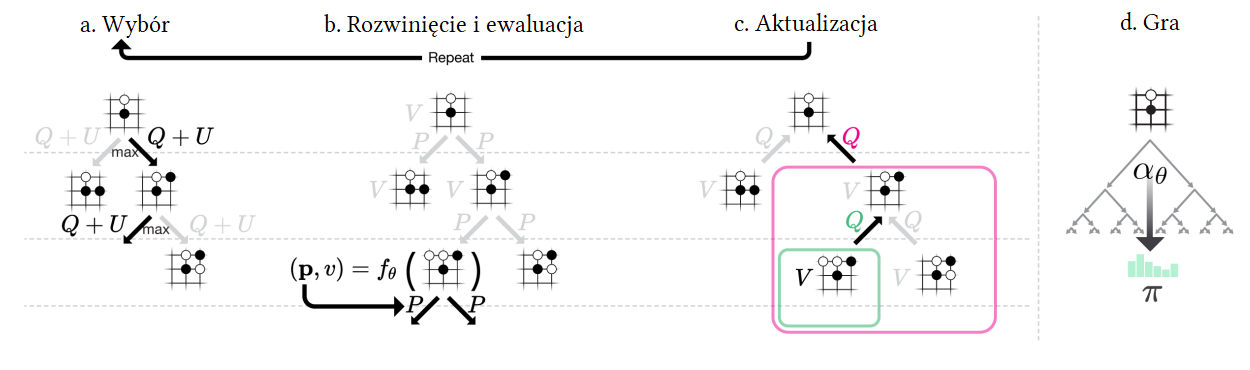
\includegraphics[width=0.8\textwidth]{alphago-mcts}
  \caption{Wykorzystanie algorytmu MCTS. \cite{alphagozero}}
\end{figure}

\section{Metoda uczenia poprzez grę z samym sobą}

\subsection{Rozgrywanie gier}

Proces uczenia się algorytmu dzieli się na trzy, następujące po sobie etapy. Pierwszym z nich jest generowanie przykładów uczących przez wytrenowaną wcześniej sieć neuronową, która reprezentuje najlepszego gracza $\alpha_{\theta^\ast}$. Rozgrywa ona kolejne gry między sobą, zapisując przebieg oraz wynik każdego z meczów, jako ciąg wszystkich wykonanych akcji $(s_t, \pi_t, z_t)$, gdzie $s_t$ to stan gry, $\pi_t$ to rozkład akcji z strategii drzewa, a $z_t$ to zwycięzca gry. Wszystkie te wartości są z perspektywy gracza wykonującego ruch w czasie $t$.

\subsection{Trenowanie na zebranym doświadczeniu}

Po zakończonej fazie rozgrywania gier, rozpoczynane jest trenowanie sieci. W tym celu losowane są przykłady z wykonanych akcji, $(s_i, \pi_i, z_i)$, a następnie optymalizowana następująca funkcja straty:

$$ (p_i, v_i) = f_\theta(s_i) \quad
J(\theta) = \sum_{i = 1}^n \Big[ (z_i - v_i)^2 - \pi_i^T \log p_i + c \lvert \lvert \theta \rvert \rvert^2 \Big]
$$

gdzie $c$ jest współczynnikiem regularyzacyjnym, a $n$ to rozmiar batcha. Celem uczenia naszego aktora jest zbliżenie strategii sieci neuronowej do strategii drzewa, uzyskanej za pomocą algorytmu MCTS, oraz dokładne przewidywanie które stany są wygrywające, a które przegrywające. Do obydwu celów dążymy jednocześnie dzięki umieszczeniu odpowiednich składników w funkcji celu. Błąd aktora jest minimalizowany za pomocą cross entropii, a krytyka za pomocą błędu średniokwadratowego.

\subsection{Ewaluacja wyuczonej strategii}

W trakcie uczenia się sieci, co pewien czas wykonywana jest ewaluacja wytrenowanego agenta, która polega na rozegraniu pewnej ilości gier pomiędzy nim a najlepszym graczem $\alpha_{\theta^\ast}$. W przypadku gdy stosunek gier wygranych przez nowego agenta przekroczy ustalony poziom, wynoszący 55\%, to staje się on nowym najlepszym graczem, a dalszy trening jest przerywany i rozpoczynana jest kolejna epoka.


\begin{figure}[ht!]
  \centering
  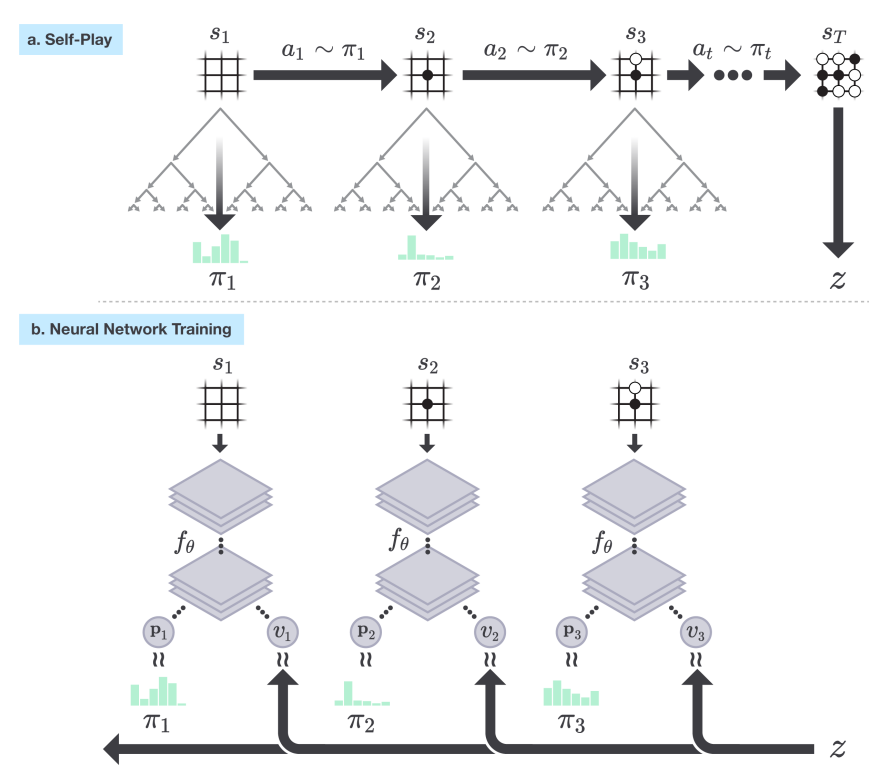
\includegraphics[width=0.8\textwidth]{alphago-self-play}
  \caption{Uczenie sieci na podstawie gry ze samą sobą. \cite{alphagozero}}
\end{figure}

\newpage

\section{Pierwsze testy na zmniejszonej planszy}

W celu dostosowania hiperparametrów algorytmu, pierwsza jego wersja była uczona na pomniejszonej planszy o rozmiarach 4 x 6. Starałem się wówczas wyznaczyć ile minimalnie gier powinno zostać rozegranych w celu wygenerowania danych uczących dla obecnej iteracji, aby model mógł dokonywać rzeczywistych postępów i wykonywać poprawną generalizację. Wyznaczenie tego było istotne gdyż czas trwania jednej epoki jest rzędu kilku dni nieustannej pracy komputera z kartą graficzną. Ponadto dobrałem wówczas również architekturę sieci neuronowej oraz pozostałe hiperparametry takie jak temperatura $\tau$ czy stała eksploracji $c_{puct}$.

Architektura sieci została ustalona na 8 bloków rezydualnych, każdy o szerokości 128 filtrów. Na każdą epokę rozgrywane było 2048 gier, w których na każdy ruch przypadało 700 rozwinięć podczas przeszukiwania drzewa i w efekcie wykonanie jednej epoki zajmowało średnio 12 godzin. Początkowy stosunek wygranych douczonej sieci przeciwko jej pierwotnej wersji jest bardzo wysoki, a z czasem zaczyna maleć, a sam proces uczenia zaczyna zwalniać i wymagane jest zwiększanie ilości gier oraz rozwinięć. Istotna okazała się również obserwacja rzeczywistego poziomu eksploracji drzewa, aby odpowiednio dostosować hiperparametry odpowiedzialne za eksploracje, gdyż przy ich złym wyborze algorytm wciąż podążał tą samą ścieżką, a w wyniku nie zdobywał nowego doświadczenia. Kod źródłowy jest dostępny pod adresem: https://github.com/mizworski/AlphaSoccer.


\subsection{Ruchy wyuczone przez model}

Sieć bardzo szybko wyucza się otwarcia, nazwanego przeze mnie dwoma rombami. Zagranie to jest w pełni symetryczne i powoduje zablokowanie przeciwnika po jego stronie boiska, z perspektywy gracza rozpoczynającego grę. Model niestety preferował rozpoczęcie gry w lewo, pomimo oczywistej symetrii planszy. Zjawisko to jest niepokojące, gdyż idealny model nie powinien rozróżniać stron i z tym samym prawdopodobieństwem, losowo wybierać jeden z symetrycznych ruchów. Remedium na to było zastosowanie przez zespół DeepMind w 2016 \cite{alphago2016} roku augmentacji danych, polegającej na wyborze losowego z 4 odbić symetrycznych planszy podczas wyboru decyzji. Jednak w późniejszej wersji, tj. AlphaGo Zero \cite{alphagozero}, zrezygnowano z tego podejścia i plansza nie była modyfikowana przed przekazaniem jej do sieci neuronowej.


\begin{figure}[ht!]
  \centering
  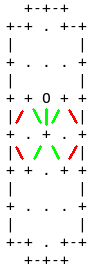
\includegraphics[width=20mm]{romb}
  \caption{Otwarcie dwóch rombów.}
\end{figure}

W momencie gdy sieć znajdowała się w jednym z pól narożnych wewnątrz boiska, obok swojej bramki, to blokowała ona kolejny ruch, aby uchronić się przed bramką. Można wówczas zaobserwować, że rozumie ona iż jeżeli chce ona wygrać, to nie może wcześniej przegrać, więc na równi ze strzeleniem gola traktuje ona obronę swojej bramki.

\begin{figure}[ht!]
  \centering
  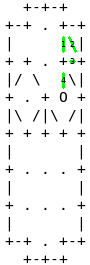
\includegraphics[width=20mm]{blok}
  \caption{Blokowanie dojścia do własnej bramki.}
\end{figure}

\begin{figure}[ht!]
  \centering
  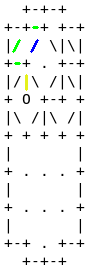
\includegraphics[width=20mm]{blok2}
  \caption{Sieć wykonała ruchu zielone, a później żółty, blokując tym samym dojście do własnej bramki. Gdyby zdecydowałą się wykonać ruch niebieski oraz żółty, to zostawiłaby przejście dla przeciwnika, który mógłby skończyć grę idąc po ukosie w lewo (7), a później dwa razy w prawo (1).}
\end{figure}

Ponadto powyższe przykłady pokazują, że sieć bez problemu rozpoznaje miejsca, w których otrzyma ona dodatkowy ruch i wykorzystuje tę wiedzę podczas planowania.

Sieć otrzymana w wyniku powyższego eksperymentu potrafiła mniej więcej w połowie przypadków pokonać ludzkiego testera.

\begin{figure}
\centering
\setlength{\tabcolsep}{5mm}
\begin{tabular}{cccc}
  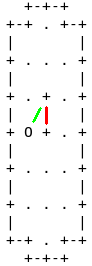
\includegraphics[width=25mm]{small0} & 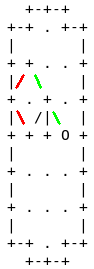
\includegraphics[width=25mm]{small1} & 
  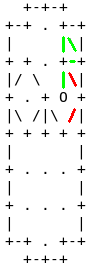
\includegraphics[width=25mm]{small2} & 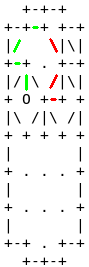
\includegraphics[width=25mm]{small3} \\
  1. 0 5 & 2. 71 33 & 3. 17 0364 & 4. 617 6524 \\[6pt]
\end{tabular}
\begin{tabular}{ccc}
  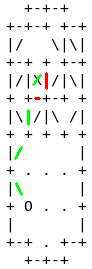
\includegraphics[width=25mm]{small4} & 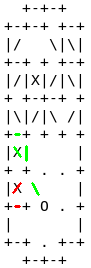
\includegraphics[width=25mm]{small5} &
  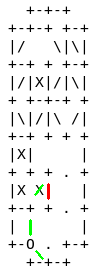
\includegraphics[width=25mm]{small6} \\
  5. 20 5453 & 6. 61 7243 & 7. 0 543
\end{tabular}
\caption{Gra pomiędzy dwoma różnymi modelami gracza na zmniejszonej planszy. Ruchy gracza wykonującego pierwszy ruch zaznaczone są na czerwono, a drugiego na zielono. Gracz zielony, który jest późniejszą wersją AlphaSoccer, wygrywa pomimo wykonywania ruchu jako drugi. }
\end{figure}

\section{Wyniki dla gry standardowych rozmiarów}

Po uzyskaniu pierwszych efektów w grze na zmniejszonej planszy, eksperymenty zostały przeniesione na pełnowymiarową planszę Przy zachowaniu tych samych hiperparametrów, pojedyncza epoka trwała już 40 godzin nieustannej pracy komputera. Testy były wówczas bardzo kosztowne, a przeszukiwanie parametrów stało się bardzo ograniczone. 

Model po paru epokach zaczął już rozumieć zasady gry i starał się przesunąć piłkę jak najbliżej bramki swojego przeciwnika. Lokalnie na planszy jego ruchy wyglądały na przemyślane i przypominały grę normalnego gracza. Nie potrafił on jednak obronić się przed bardzo długimi ruchami, tj. takimi w których wykonywane było wiele odbić. Ostatecznie wystawiał się on na tego typu ruchy, które prowadziły do jego porażki.


\subsection{Gra pomiędzy wczesną i późną iteracją modelu}

Rozgrywki średnio zawierają aż 100 ruchów, rozłożonych na około 20 rund, co sprawia że ich wizualizacja staje się bardzo ciężka. Poniżej przedstawiam zapis jednej z rozgrywek w standardowej notacji oraz kilka plansz po zakończonej grze.

\texttt{1.\,0 5\;
2.\,0 33\;
3.\,1 3\;
4.\,17 54\;
5.\,7 45\;
6.\,0 3\;
7.\,16677 5\;
8.\,0 3\;
9.\,17 55253\;
10.\,1 3\;
11.\,1177 543\;
12.\,11 3664633\;
13.\,1 3\;
14.\,170 35\;
15.\,717 5066666336\;
16.\,3 5\;
17.\,7244 30\;
18.\,752712142227442 3\;
19.\,17575 3\;
20.\,06764 3\;
}

\begin{figure}
\centering
\setlength{\tabcolsep}{5mm}
\begin{tabular}{cccc}
  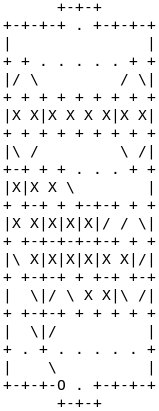
\includegraphics[width=35mm]{standard0} & 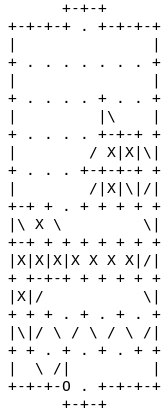
\includegraphics[width=35mm]{standard1} & 
  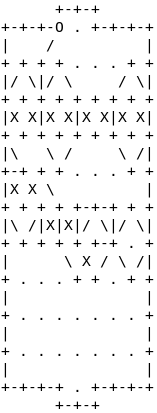
\includegraphics[width=35mm]{standard2}\\
\end{tabular}
\begin{tabular}{ccc}
  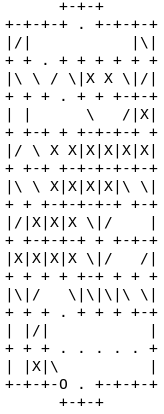
\includegraphics[width=35mm]{standard3} & 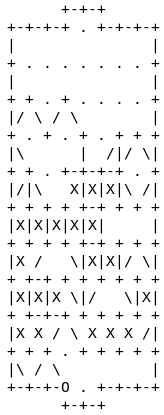
\includegraphics[width=35mm]{standard4} \\
\end{tabular}
\caption{Plansze po ukończonych rozgrywkach na pełnowymiarowym boisku.}
\end{figure}

\chapter{Wnioski}

Wytrenowanie algorytmu zdolnego do gry w dowolną planszową grę strategiczną jest obecnie możliwe przy użyciu znanych nam technik, jednak okazuje się być poza zasięgiem przeciętnego człowieka, który nie dysponuje zapleczem obliczeniowym takim jak DeepMind czy OpenAI. Karta graficzna z najwyższej półki obecnie jest zdolna do wykonywania około 8~gigaflopsów, to jest $8 \cdot 10^9$ operacji zmiennoprzecinkowych na sekundę (flops, ang. floating points operations per second). Do określenia ilości operacji wykonanych podczas pełnego wytrenowania sieci neuronowej wykorzystuje się jednostkę \emph{petaflopso-dni} i jest to ilość operacji wykonanych przez maszynę o wydajności 1 petaflopsa ($10^{15}$ flops) przez cały dzień. 

\begin{figure}[ht]
  \centering
  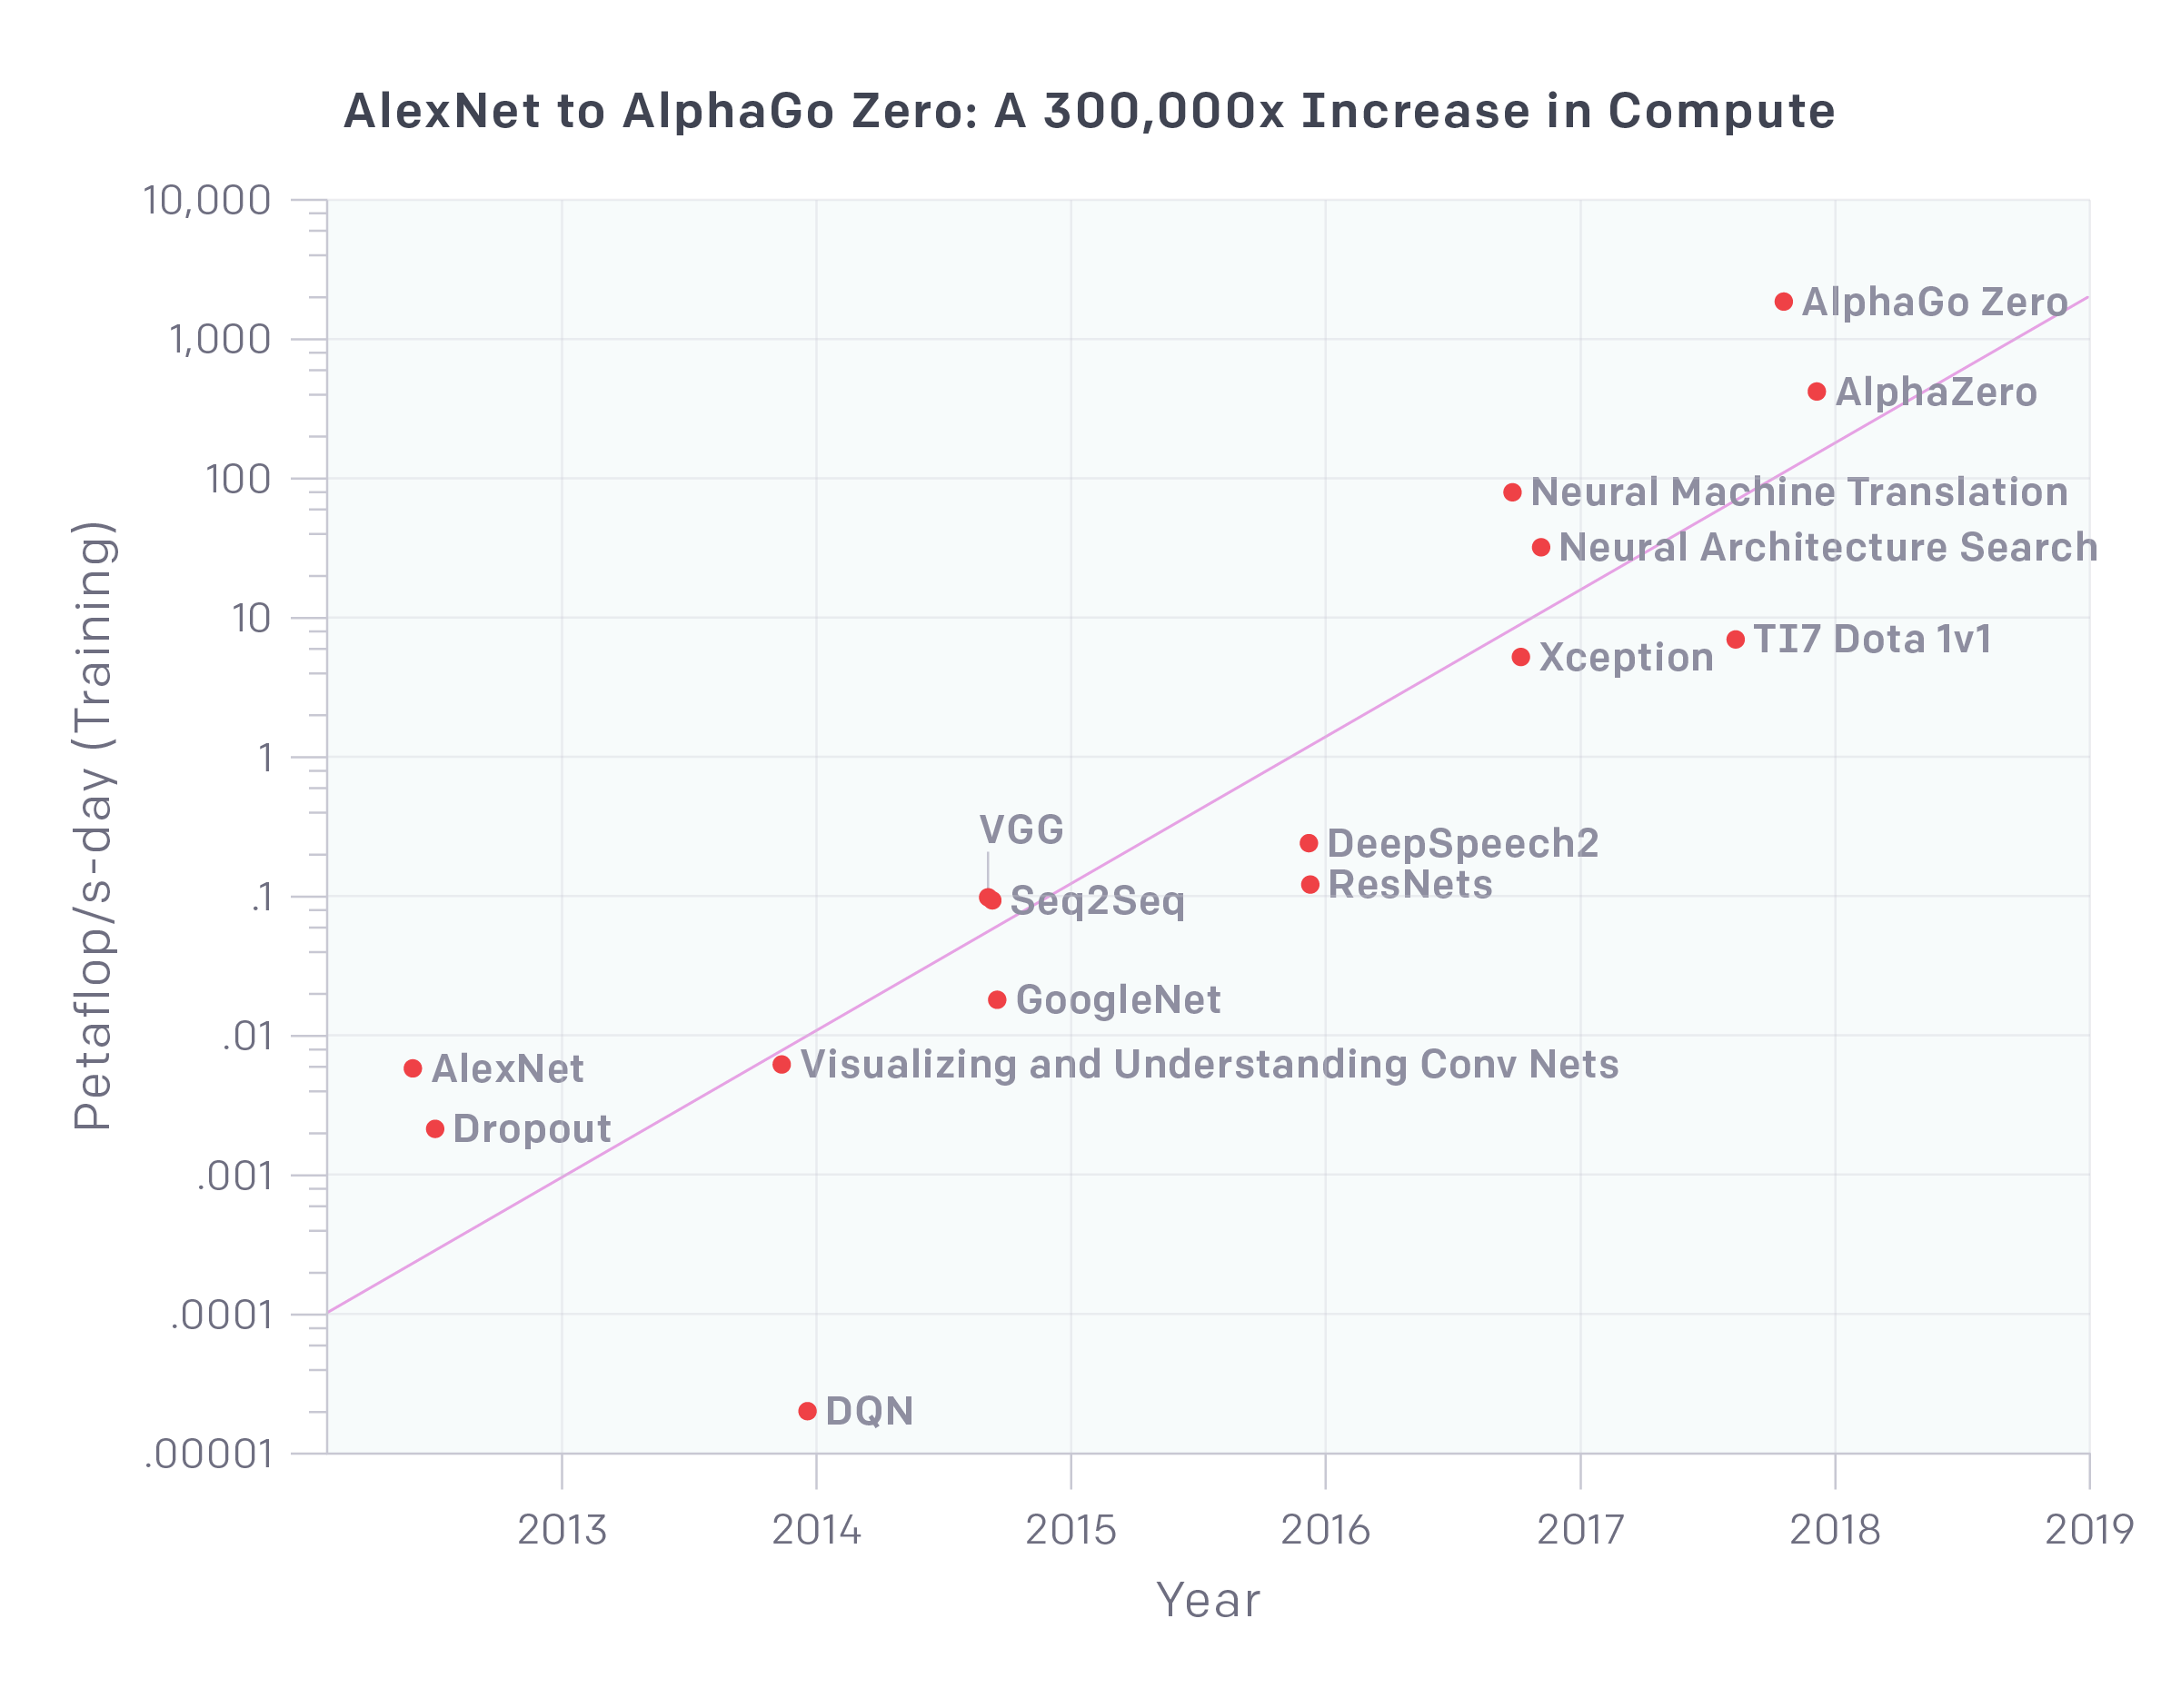
\includegraphics[width=0.8\textwidth]{compute}
  \caption{Ilość petaflopsodni wykorzystanych podczas poszczególnych projektów \cite{dqn, resnet, dota2, nmt, alphago2016, alphagozero}}
\end{figure}

Obecne problemy z którymi zmagają się specjaliści od uczenia ze wzmocnieniem wykorzystują dziesiątki, setki, a nawet tysiące petaflopsodni \cite{openai-compute}. Przeciętna karta jest o rzędy wielkości poza zasięgiem zbliżenia się do tych wartości. Na wykorzystanie tych algorytmów do celów niekomercyjnych będziemy musieli jeszcze trochę poczekać.

Kontrolowanie procesu uczenia okazało się niezwykle istotne podczas wykonywania tego eksperymentu. Warto sprawdzać czy rozkłady prawdopodobieństw dla akcji wykonywanych przez trenującego agenta oraz tworzone przez niego oceny stanów są zgodne z naszą intuicją. Dodatkowo warto też śledzić rozgrywane gry, aby wyłapać ewentualne dziwne zachowania. Łatwo jest popełnić błąd, który nie prowadzi do przerwania wykonania programu, jednak zasadniczo utrudni uczenie lub uczyni je kompletnie bezsensownym.

Na początku procesu uczenia może nam się błędnie wydawać, że nasz agent dokonuje postępy, gdy w rzeczywistości będzie to losowy szum. W tym wypadku pomocne okazuje się testowanie agenta przeciwko strategii wykonującej losowo akcje. Warto również znaleźć metrykę, która pozwoli nam na obiektywną ocenę umiejętności naszego algorytmu, np. punkty elo.

Podczas implementacji algorytmu powinniśmy dokładnie weryfikować wszystkie założenia, które poczynają autorzy prac z których korzystamy i weryfikować czy w dobry sposób je interpretujemy. Zazwyczaj zawierają one wiele, dobrze ukrytych szczegółów, których nie uda nam się wyłapać za pierwszym razem, gdy czytamy dany tekst. Warto zatem od czasu do czasu ponownie przeczytać opracowywane teksty, aby upewnić się, że wciąż utrzymujemy się na poprawnym kursie.

Błędy w kodzie mogą być dla nas bardzo kosztowne, gdyż może się zdarzyć że przeprowadzimy serię różnych eksperymentów, w celu ustalenia optymalnych hiperparametrów. Jednak po znalezieniu i naprawieniu błędu, może się okazać że zachowanie modelu jest zupełnie inne, a w konsekwencji będziemy musieli powtórzyć wszystko co zrobiliśmy do tej pory.

Rozwój sztucznej inteligencji w ostatnich latach w większości dotyczy bardzo wąskich zastosowań. Modele do rozpoznawania obrazów czy tłumaczenia tekstów potrafią rozwiązywać tylko swoje wyspecjalizowane zadania i bardzo daleko jest im do traktowania ich jako rozumne twory. Najbliższe ogólnej sztucznej inteligencji (ang. Artificial General Intelligence, AGI) obecnie są właśnie algorytmy uczenia ze wzmocnieniem, których interakcja z otoczeniem najbardziej przypomina inteligentne zachowanie. Jednak nawet im jest daleko, abyśmy mogli uznać je za niezależne istoty, które potrafią zrozumieć otaczający je świat i wykształcić świadomość. Nie mniej jednak z entuzjazmem podchodzimy do rozwoju tej dziedziny, aby przybliżyć nas o kolejny krok do AGI.


%\begin{thebibliography}{99}
%\end{thebibliography}


\bibliographystyle{acm}
\bibliography{bibliografia}

\end{document}


%%% Local Variables:
%%% mode: latex
%%% TeX-master: t
%%% coding: latin-2
%%% End:
